%% project-plan-st1-en.tex

%% Copyright notice:
%% Copyright (C) 2013 Aarón Bueno Villares

%% Source package notice:
%% This file is part of the FreeAlgView-project-doc package. You can get this
%% package in zip and tar.gz formats in the next url:
%%
%%  - https://github.com/Peregring-lk/FreeAlgView-project-doc/downloads

%% License notice:
%% The FreeAlgView-project-doc package is made available under the terms of the
%% Creative Commons Attribution-ShareAlike license, either version 3.0 of the
%% license, or (at your option) any later version. You can read this license in
%% the next url:
%%
%%  - http://creativecommons.org/licenses/by-sa/3.0/
%%
%% See also the LICENSE.txt file at the top-level directory of this package or
%% in the next url:
%%
%%  - https://github.com/Peregring-lk/FreeAlgView-project-doc/blob
%%    /master/LICENSE.txt

\documentclass{article}

\usepackage[english, nofullpage, nolicensec]{./fav-project-headers/fav-headers}

\title{\fav: Oct 2012 - Sep 2013 Final Report}
\author{Aarón Bueno Villares \textit{$<$abv150ci@gmail.com$>$}}
\datelicense{\today}

\setcounter{tocdepth}{2}

\begin{document}

\maketitle

\begin{abstract}
  In this report it will be presented the actual state of \fav v0.5, a ``libre
  and learning-oriented algorithm animation application'', containing a
  relatively detailed description about the developed language, \faupp, and the
  core module of the application, with special attention to memory management
  and the \texttt{henfo} concept, trying to justify each design issue with lot
  of reflections. Before getting into technical details, it is also given a
  general discussion about algorithm animation systems and its general
  properties.
\end{abstract}

\tableofcontents

\section{Introduction}
This document represents a review of the work made during the academic year the
project has been developed, from October 2012 to September 2013. This time
represents a complete Erasmus stay in the \textit{Fachhochschule
  Würzburg-Schweinfurt}, Germany, being my home university the
\textit{Universidad de Cádiz}, Spain.

Concisely, the achieved goals are the followings:

\begin{description}
  \item[Programming environment] Designed and implemented different concepts
    used throughout the application, like those used to manage memory
    management, useful and comfortable \textit{C++} idioms and nodes.
  \item[Algorithm/animation dilemma] Found a way of designing a language for
    solving the dilemma about machine and human semantic levels.
  \item[Language design] Designed a suitable language for the need of \fav, with
    a working grammar and successful generation of its parser tree. The name of
    that language is \faupp.
  \item[Interpreter implementation] Implemented the basic process of computation
    and behaviour of \faupp.
\end{description}

The current \fav and \faupp version is v0.5.

\section{Definition and scope of \fav}
\fav is, respectively, a ``libre and learning-oriented algorithm animation
application''. ``Libre'' means here ``free as freedom, NOT as free beer'' as
Richard Stallman states. Additionaly, the project is licensed under the terms of
the GNU General Public License version 3. ``Libre'' is the Spanish and French
translation of the word ``free'', choosed by the Free Software Fundation to
avoid the ambiguity cited above. Being ``learning-oriented'' means the first
purpose of \fav is to make easy to understand algorithms, by means of custom and
suitable animations. Learning-oriented systems should be distinguished from
teaching-oriented systems, which are only for teachers or professors, but not
directly by students. So, that excludes self-learning. In contrast, \fav is
oriented to anybody who wants to learn or understand algorithms. The way the
``application'' does it is by means of ``animations''. With this paragraph, all
parts of the definitions are already justified. The language used to implement
\fav is C++, and the graphic engine is Qt. The software tools and libraries used
to develop \fav has been choosen to make \fav multiplatform, like, among others,
\textit{Qt} or \textit{bisoncpp} (a tool extending \textit{bison} to add
object-oriented capabilities).

The central service or purpose of \fav is, then, to allow you writing
algorithms and custom animations for them in an adequate and comfortable
way. Since the language is also a graphic one, it allows you in consequence
creating animations or drawing scenes of any other type or nature, with
independence of an algorithm if wanted, but this is an optional or extra feature
(you can use it of this way if you want, but that is not the main purpose of
\fav, only a natural consequence of how \fav works).

\subsection{Justification}
\label{ssec:justification}
\vspace*{-2ex}\hspace*{3.4em}\textit{\scriptsize{$\rightarrow$ First paragraph
    from the \favc}}

Facilitating learning is the key issue to accelerate the professional
formation. Specialization is increasingly important and consumes more
and more time. But it is also important to ensure the quality of this
education. Bibliography related to algorithm visualization
software states the visualization together with textual explanations
improves substantially the retention of the students studying a
certaing algorithm. In the other hand, motivation is the
principal requirement in the success of the learning process. An
application making easier the knowledge can increase the motivation of
students while constitutes an advantage to learning, and thus the
quality of the whole learning process is increased.

Furthermore, among all current algorithm animation or visualization systems and
other related system available in the ``jungle of Internet'' or founded in the
literature, there isn't any system that meets the thinking traits for \fav. The
most modern systems have built-in algorithms and data structures and can't
animate any other algorithm or data structure. The most complex thing you can
make with these systems is to change values of parameters or go steps forward
and backward in the execution process. Others systems (a few) offer an
interpreted language and you can write your custom algorithms, but they only
draw a ``simulated machine'', so, these animations depict behaviours of
algorithms on a machine's semantic level, but no on a \textit{algorithm}'s
semantic level, because it's impossible for a computer to extract automatically
the semantic of an algorithm. That will be explain more concisely in section
\ref{ssec:problem}.

Other systems aren't libre, or are so old that they have been
abandoned. Finally, other systems capable of animating or showing somehow any
algorithm, aren't simple enough to be a learning tool, due to they work by means
of calls to system's graphic routines, for example, inside a C program that
contains your algorithm, programmed also in C.

Thus, there isn't any application or system satisfying the described needs,
which will be subject of \fav.

\subsection{Problem to be solved}
\label{ssec:problem}
The service that \fav offers is a way of writing algorithms and executing and
drawing them. But the real complexity behind this service is related to the
ideas stated in the last paragraph of the previous section. It can be said an
algorithm has two ``semantic levels'':

\begin{description}
  \item[Algorithm level] The semantic of the algorithm's itself: what is the
    purpose of the algorithm, what problem solves, what is the relation between
    inputs and outputs, which properties it has, or how its behaviour or
    executing process work.
  \item[Machine level] A language has always a related machine, as a formal set
    of variables, in a more mathematical point of view, whose value represents a
    machine state, and the \textit{semantic of the language} is how the
    execution of each syntactic element changes the state of the machine. So,
    the machine semantic level of an algorithm is how each sentence or
    instruction of that algorithm changes the machine state, according to the
    defined semantic for each syntax element of the language which was used to
    write it.
\end{description}

So, while the machine semantic level of the algorithm can change if the
algorithm is now expressed in a different language, its ``algorithm'' or human
semantic level doesn't change, because it solves the same problem.

With these definitions clear, we can accordingly express better what is the real
problem behind the services \fav tries to offer, and why the currently available
systems which offer the same service, have the properties they have. We have said
there are fundamentally two systems (the first one more common that the second):

\begin{description}
  \item[Operating at algorithm level:] They are the most modern ones (normally
    Java applets), with pre-implemented algorithms, but suitable animations,
    allowing you to understand easily how these algorithms or data structures
    work, but without possibility of writing your custom algorithms. Two pages
    with a large list of applications of this category can be found in
    \cite{inaction} and \cite{galles}.
  \item[Operating at machine level:] I call them, ``debugger-like'' systems. You
    can write any algorithm you want, inside the limits of the language given by
    the system, and the system draws, in a suitable way, the machine itself,
    showing the set of defined variables, remarks about the current instruction,
    and controls for going steps forward or backward, as well as changing
    parameters. The title ``debugger-like'' makes reference to real graphical
    debuggers, which mission is to show in a graphical interface, how the state
    of the internal machine changes for each instruction. It is fair to say
    there is very few systems of this type. The best founded software of this
    category is \textit{UUhistle}\cite{uuhistle}.
\end{description}

So, you have two possibilities: to understand well the behaviour of only a
concrete algorithm, or understand good only the behaviour of the machine (for
any algorithm). Is there any current system which makes available for you both
possibilities? I have found no one, and there is a very good reason for that:
its impossible for a machine to extract automatically the ``semantic'' of an
algorithm; that is an exclusive capacity of human beings. Other older systems,
the oldest ones actually, like \textit{BALSA}\cite{balsa} or
\textit{TANGO}\cite{tango} and their sucessors, work by means of annotating
programs, sending or notifying about events in key points of the target program,
and making graphic calls to a library within the same program, or communicating
somehow with an external system, but the library or the system itself doesn't
know anything about the executed program and its real current state. That is
indeed a ``complete'' way or solution to write algorithms, from the point of
view of offering the posibility to create custom animations for any algorithm,
but with the disadventage of not being able to offer you any other type of
information apart from the supplied by these annotations, which is not flexible
enough.

For more information, visit the portal AlgoViz.org\cite{algoviz}. It is a
``gathering place for users and developers of algorithm visualization and
animations'', founded and supported by the National Science Foundation, and it
contains, in its section \texttt{AV Catalog}, the hugest list of applications
about algorithm visualization I have ever found. It contains about 850
applications in its list. A concise history about algorithm animation can be
also found in \cite{hist}.

\subsection{Found solutions}
Seeing this contradiction between these two semantic levels of an algorithm, it
is obvious if I want to create a visualization system that works with any
algorithm, I should be close to the first type of systems, those which work in a
``machine level''. So, I need at least a programming language together with an
interpreter which executes any function or piece of code written in that
language, over a machine. After that, the next step is how I make available to
users a way of creating visualization or animations for it. An automatic
visualization, we have seen, is impossible to offer if we want a useful system
to understand it in a ``human level''. So, some solutions were coming to my
mind, all of them with a common characteristic, to create a second language for
specifying animations:

\paragraph*{A descriptive language}
A descriptive language is a language which doesn't use ``instructions'' or pieces
of computation. They are only useful to specify data or properties. Famous
examples of descriptive languages are:

\begin{description}
\item[HTML:] A language to describe, by means of ``tags'',
  properties of a piece of text of a web page, like style (blod, italic) or
  size (10pt, 12pt), scope of paragraphs, lists, enumerations and other
  ``itemize'' environments, backgrounds and colors, and so on.
\item[XML and its dialects:] A generalization of HTML for adding any type of
  marks to a piece of text, or in a more general point of view, for defining a
  structure or hierarchy of information.
\item[Wiki markup:] The language used by the software MediaWiki for formatting a
  page, with same purpose as HTML. The most universal well-known system using
  MediaWiki is the encyclopedia Wikipedia.
\item[QML:] Language of the Qt framework to design graphic user interfaces of a
  (Qt) application, by means of specifications of the graphic elements the
  application has, available actions or, even, animations by means of
  descriptions of each one of its steps.
\end{description}

My first attemp was to use a declarative language like the cited ones above to
specify somehow properties of an algorithm or any other continuous piece of code
which it is required to be animate. This language would have different resources
for specifying the different properties an animation could need, like circles,
rectangles, text, position, organization of the screen (layouting), colors,
background, fonts, and so on. This language would be written in a different file
for not poluting the algorithm (improving readability and ease of modification
of the algorithm itself), and would offer a way to specify these properties and
over which parts or sentences of the code they would be applied.

It is fair to say this language revives actually the oldest systems like
\textit{BALSA} or \textit{TANGO} (cited in the section \ref{ssec:problem}),
since the idea is to annotate programs, but at that time, when I was designing
this language, I didn't actually know how these systems exactly work. But
otherwise, \fav wouldn't resemble to these systems since \fav knows which
algorithm it executes, with all the adventages this has, as will be seen
throghout the rest of this report.

The thought implementation of that language was by means of an annotated
``syntax tree''. So, the parser would read the file describing the algorithm,
would create its syntax tree, and after that, the file describing its animation
would be read, and the syntax tree would be annotated with the information
specified in that second file. Each node could has one or more
annotations. After that, the system would execute that syntax tree to compute
the algorithm (using the parameters specified by the user) and each time an
annotated node is reached, the system would draw something according to that
annotation. So, the animation would be the product of the sequence of founded
annotations, plus a serie of controls to control the steps or to change of
parameters.

In order to simplify writing, annotations were planned to be also inherits from
parents to children, as depicted in the figure \ref{fig:annonst}. How these
annotations could be added to at specific node in a elegant, extensible,
reusable and scalable way brought me to create the ``henfo'' concept, explained
in section \ref{ssec:henfo}, concept that I'm still using for \fav.

\begin{figure*}[h!]
\begin{center}
  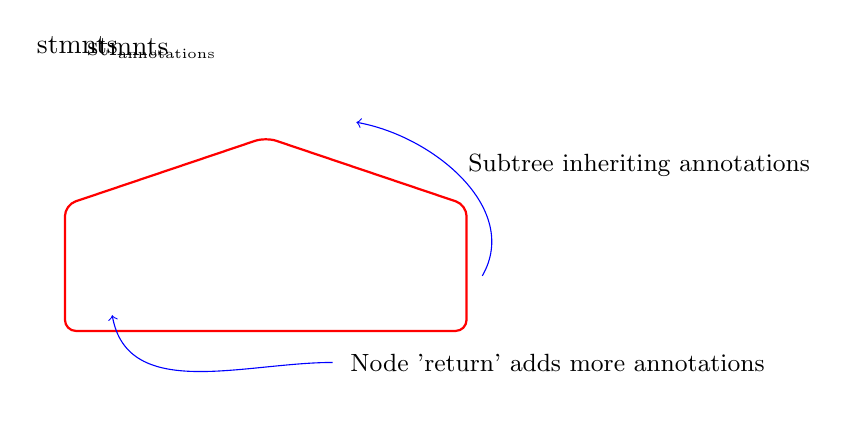
\begin{tikzpicture}[%
      sibling distance=.5cm,
      label/.style={font=\footnotesize\color{red!70!black}}]
    \Tree
        [ .translation\_unit [ .stmnt assign ]
          [ .\node(ref){stmnts${}_{\mbox{\tiny annotations}}$}; [ .stmnt
              return${}_{\mbox{\tiny annotations}}$ ] [
              .\node(child){stmnts}; \edge[roof]; {more stmnts} ] ] ]

        %\draw[semithick,->] (child)..controls +(norht est:5) and
        %+(est:5)..(ref);

        \coordinate (O) at (1.75, -1.14);
        \coordinate (OM) at (2.9, -0.95);
        \coordinate (L) at (-0.8, -2);
        \coordinate (R) at (4.3, -2);
        \coordinate (LL) at (-0.8, -3.6);
        \coordinate (RR) at (4.3, -3.6);
        \coordinate (MR) at (4.5, -2.9);

        \draw[red, thick, rounded corners] (O) -- (L) -- (LL) -- (RR) -- (R) --
        cycle;

        \draw[blue,->] (MR) to[out=60, in=350] (OM);
        \draw[blue,->] (2.6, -4) to[out=180, in=280] (-0.2, -3.4);

        \node[right] at (4.2, -1.5) {\small{Subtree inheriting annotations}};
        \node[right] at (2.7, -4) {\small{Node 'return' adds more annotations}};

  \end{tikzpicture}
\end{center}
\caption{A sample annotated syntax tree}
\label{fig:annonst}
\end{figure*}

The problem of these types of languages are precisely that lack of computational
power, since descriptive language has nothing. Different nodes could need
different conditions to be meet before applying an annotation, and this implies
to have, at least, some computation power to deal with variables, logic
operations and conditions. Moreover, working with a descriptive language implies
all possible user actions (clicks, mouse movements or key strikings) have an
implemented predefined and not customizable behaviour, or customizable by means
of a user menu, but this is in all respects necessarily limited, especially if
an algorithm works with complex structures and requires complex and specific
actions for interacting with users, like contracting nodes of a tree, custom
layouts or hiding of screen sections, or steps forward and backwards based
on conditions, number or iterations, number or calls or whatever useful tool for
helping better understand the algorithm, the key purpose of the system.

\paragraph*{Programming languages}
The most customizable behaviour you want for a system, the most close you are to
implement a programming language for it. And this was exactly the next approach,
two programming languages, one for describing algorithms (which will be called,
the ``programming language''), and another for programing actions and animations
animating and interacting with them (which will be called, the ``graphical
language''), by means of graphical primitives in the language. So, the
plannification of the system was growing up to a more general one. Naturally,
this implies to achieve longer-term goals, for a more powerful system.

Once determined for having two languages, the next step was to ask about the
features of these new languages. While the ``programming language'' can be
relatively simple, because algorithms in an educational point of view are more
conceptuals, the graphical language should be complexer. For example, if you
want to make animations for algorithms performing computations over trees or
graphs, you need the graphic language can also work with these types of
structures. Also it would need event-oriented features, because events are a key
issue in graphical applications.

Given that we do already have a complete programming language with graphical
capabilities, the system itself doesn't necessarily have to define any
pre-implemented feature or element of the GUI, delegating them to the graphical
language itself. Now, actions associated with mouse events, responses to
keystrokes, boxes to input parameters, controls, or the layout of the screen,
can now be programmed directly by the graphical language. Of course, this
implies the language should be suitable for reusing code, for working with
larger programs, it should have a fast implementation to perform a good user
experience, and so on. We can say that we have to create a language for real
purposes, with higher expectatives. And the best programming paradigm to work
with such a type of complexity is the object-oriented paradigm, mainly for the
adventages inheritance and type polymorphism have.

Another consequence is users (in a general point of view) have more
responsabilities than before, but this can be solved by means of standard
packets, third-parties code, startup-files, and any other recurse real
environments for interpreted languages have.

Last reflection: if I have two programming languages, why not having only one?
I doesn't have to design, develop and maintain two languages and interpreters,
having both languages a complete computational power (Church-Turing tesis). This
would be stupid!

We can not also forget the first purpose of the language: drawing or animating
algorithms, and for this reason the language should have also features for
making easy to do it. Some questions arise:

\begin{itemize}
\item Where is the border or frontier between ``algorithm'' and ``animation'' if
  we have now only one language?
\item How can I create a ``comfortable language'' for writing algorithms, and at
  the same time, for doing complex things?
\item Is it really necessary to work at this level of complexity?
\end{itemize}

If you read carefully again this section, you can see we have opened more
questions than those we was intending to solve. But this is the common procedure
for solving any problem! The original problem is granulated on more concrete
questions once you have an ``hypothese'' about how you can solve it, solutions
of these more concrete questions come recursively with even more concrete
questions, whose final answers bring you to the final solution of your original
problem. The following sections will try to put order in this question-chaos,
explaining more carefully how this language works, how it looks like, which
optimization solutions has been found, solving all questions put on the table,
and finally, justifying why we should work with such a complex and complete
language.

\section{Language basic architecture}
In this section it will be explained the basic architecture of the language and
how I pretend to implement the way the ``algorithm'' and ``animation'' parts of
the language communicate themselves. The name of this language is
\faupp. \textit{Fau} is an acronym of \fav, substituying ``v'' by ``u'' to make
the acronym pronunciable. Its postfix, \textit{pp}, makes reference to
\textit{plus plus} imitating \textit{C++}, my first and predilect language.

\subsection{Definitions}
In this section some definitions, which we will need for the following sections,
will be clarified. Not all concepts of this report will be defined here, because
many of them are more technical and it is better if they are defined in its
corresponding section. We can say these definitions correspond to basic
vocabulary.

\begin{description}
  \item[Source code] Source code receives here its natural interpretation: the
    source code of \fav is the C++ implementation of \fav itself.
  \item[Application] It makes reference to \fav. It's the output of the ``source
    code'' after its compilation.
  \item[User code] Any portion of code written in the \faupp language.
  \item[Parser] The subsystem of the application which purpose is to transform
    the user code to a syntax tree.
  \item[Interpreter] The subsystem of the application which purpose is to
    execute or interpret source code, once transformed to a syntax tree by the
    parser, with an additional previous step to construct the machine
    itself. \fav is currently 80\% the interpreter, since other objects or
    modules, like memory management, or the parser itself, are always called or
    used directly of indirectly by the interpreter, since the interpreter
    ``rules'' or ``domains'' the main loop of the application.
  \item[Computation or execution] The computation or the execution is what the
    interpreter makes. The word ``computation'' is used in a more specific
    context as ``execution'': while ``execution'' is a way for expressing the
    complete process of running user code, with ``computation'' we express a
    more close view of the execution process, with more interest about each one
    of its steps.
  \item[Step] We understand step to each machine upload.
  \item[Programmer] A programmer is any user who writes user code. Programmer
    can also mean somebody who develops \fav itself (who writes source code),
    but since this meaning of programmer will not be really used in this report,
    we have no risk of ambiguity. If we want to use the word programmer in that
    second meaning, this will be specifically said.
  \item[Algorithm] It makes reference to any user code which purpose is
    \textbf{to be animated}, but not the user code which purpose is to animate
    something. There is no really syntactic distinction between algorithm and
    animation. The \faupp interpreter doesn't really distinguish between
    user code executing an algorithm and user code executing an animation. It
    executes all user code in same conditions, making graphical calls when it
    founds graphical routines in the user code. So, this algorithm/animation
    distinction is more semantic than syntatic.
  \item[Animation] Animation makes reference to any function or portion of user
    code with ``graphical purposes'', in contrast with \textit{algorithm}.
  \item[Designer] A programmer who writes animations. Its important to say
    programmer is a more general word than designer, or what is the same,
    designer is a more specific word than programmer. So, the word ``programmer''
    implies both designer and any other programmer.
  \item[User] A final user. Somebody who uses \fav to see already made
    animations without acting as a programmer, is a (common) user.
  \item[Program] It makes reference to the behaviour or ``program'' resulting of
    executing user code. So, the program is the output of ``what you write'' in
    \faupp. Obviously, the first purpose of \faupp is to allow you to write
    programs for animating algorithms, although in a more pragmatic point of
    view, you can use \faupp to write any type of program you want (inside the
    limits of the language, don't try to implement a web server in \faupp).
\end{description}

\subsection{The \textit{Emacs} analogy}

\textit{Emacs} is a text editor, with a curious behaviour. In the MIT
(Massachusetts Institute of Technology), in the 1970s, the tool using for
editing texts was TECO. TECO was an interpreted language whose commands allowed
you to manipulate text files. That TECO system worked by means of different
commands for opening files (without seeing its contents), searching strings
inside them (by means of regular expressions, like \textit{grep}), returning the
lines containing them, and once you had the line you wanted to modify, changing
the contents of this specific line with other commands. Richard Stallman, who
worked in the MIT, knew other new editors with WYSIWYG behaviours (\textit{What
  You See Is What You Get}) and Stallman was improving TECO during the following
years to add to TECO WYSIWYG features. In 1976, Stallman developed the first
version of the \textit{Emacs} system, which was an improvement of the TECO
system with the following characteristics:

\begin{itemize}
\item An interpreted language based on lisp, called \textit{elisp} (from
  \textit{Emacs lisp}).
\item Visualization in real time of changes made over the file you are modifying.
\item Bindings between key inputs and macros or custom commands written in
  \texttt{elisp}.
\end{itemize}

So, \textit{Emacs} works as follow: each time you type a keystroke (from
individual characters like \textbf{a} or \textbf{b} or \textbf{\char`\\ n}, to
complex bindings like \textbf{``Control-c Control-d e''} or \textbf{``Shift-a
  Meta-d q''}), a macro or function is called, this function is executed,
changing accordingly the state of the internal machine of \textit{elisp}, and
\textit{Emacs} reads the internal state of the machine to show the results. So,
each time you open a file in \textit{Emacs}, this file is transformed to a
buffer (which works as a variable of the \textit{elisp} machine), and each time
this buffer is modified (after the execution of an \textit{elisp} macro or
command), you see in real-time its consequences (for example, a change in a
file).

So, \textit{Emacs} combines the adventages of WYSIWYG editors with the
powerfulness of programming languages: with \textit{elisp} you can, not only to
execute macros to modify text, but also to call to external process (like a
compiler), to show other types of documents, like images or PDFs, to read and
write e-mails, to play text games, to chat in IRC channels, to create
screensavers for your idle time or even to surf in Internet. This is the
adventage of working with an interpreted embebbed in a text editor, that you
have a little operative system.

\begin{figure*}[h!]
  \begin{center}
    \includegraphics[scale=0.25]{images/emacs-sample.png}
    \caption{An example of Emacs session, with a little file of source code, a shell
      terminal, a buffer showing the state of compilation, and a text file with
      images.}
    \label{fig:emacsess}
  \end{center}
\end{figure*}

\textit{Emacs} is a really good example of a model-view architecture, the model
being the \textit{elisp} machine, and the view being \textit{Emacs} itself (we
can say \textit{Emacs} is the GUI). So, \fav works (designed to work) with this
architecture in mind: being the \textit{model} the state of the machine of the
programming language, and the \textit{view}, the windows showing animations,
which depends on the machine state. \fav has an important difference with
\textit{Emacs}: while the way \textit{Emacs} shows the internal state
of the \textit{elisp} machine is pre-defined (you can not modify it, and there's
no graphical routines), \fav \textbf{needs} the graphical appearance is
completely specified, since it depends on the semantic developers want to give
to the machine state, which interpretation can depend on the algorithm being
currently executed.

\begin{figure*}[h!]
\begin{center}

  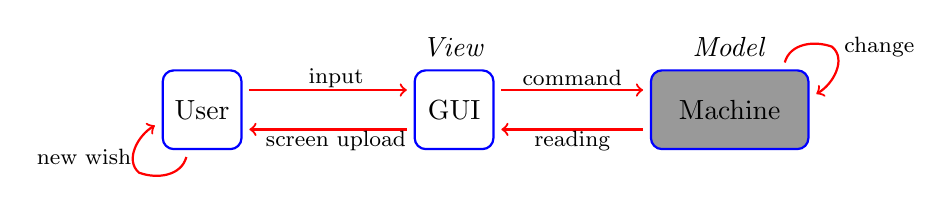
\begin{tikzpicture}

    \coordinate (UU) at (-0.2, 0);
    \coordinate (UC) at (0.3, -0.5);
    \coordinate (UD) at (0.8, -1);

    \coordinate (GU) at (3, 0);
    \coordinate (GC) at (3.5, -0.5);
    \coordinate (GD) at (4, -1);

    \coordinate (MU) at (6, 0);
    \coordinate (MC) at (7, -0.5);
    \coordinate (MD) at (8, -1);

    \coordinate (UGS) at (0.9, -0.25);
    \coordinate (UGT) at (2.9, -0.25);

    \coordinate (GUS) at (2.9, -0.75);
    \coordinate (GUT) at (0.9, -0.75);

    \coordinate (GMS) at (4.1, -0.25);
    \coordinate (GMT) at (5.9, -0.25);

    \coordinate (MGS) at (5.9, -0.75);
    \coordinate (MGT) at (4.1, -0.75);

    \coordinate (MMS) at (7.7, 0.1);
    \coordinate (MMC) at (8.3, 0.3);
    \coordinate (MMT) at (8.1, -0.3);

    \coordinate (UUS) at (0.1, -1.1);
    \coordinate (UUC) at (-0.5, -1.3);
    \coordinate (UUT) at (-0.3, -0.7);

    \draw[blue, thick, rounded corners] (UU) rectangle (UD);
    \draw[blue, thick, rounded corners] (GU) rectangle (GD);
    \draw[blue, thick, rounded corners, fill = black!40!white] (MU) rectangle (MD);

    \draw[red, thick, ->] (UGS) -- (UGT);
    \draw[red, thick, ->] (GUS) -- (GUT);

    \draw[red, thick, ->] (GMS) -- (GMT);
    \draw[red, thick, ->] (MGS) -- (MGT);

    \draw[red, thick, ->] (MMS) to[out=75, in=160] (MMC) to[out=320, in=30] (MMT);
    \draw[red, thick, ->] (UUS) to[out=255, in=340] (UUC) to[out=140, in=210]
    (UUT);

    \node at (2, -0.1) {\footnotesize{input}};
    \node at (2, -0.9) {\footnotesize{screen upload}};

    \node at (5, -0.1) {\footnotesize{command}};
    \node at (5, -0.9) {\footnotesize{reading}};

    \node at (8.9, 0.3) {\footnotesize{change}};
    \node at (-1.2, -1.1) {\footnotesize{new wish}};

    \node at (UC) {User};
    \node at (GC) {GUI};
    \node at (MC) {Machine};

    \coordinate (GT) at (3.5, 0.3);
    \coordinate (MT) at (7, 0.3);

    \node at (GT) {\textit{View}};
    \node at (MT) {\textit{Model}};

  \end{tikzpicture}

  \vspace*{5em}

  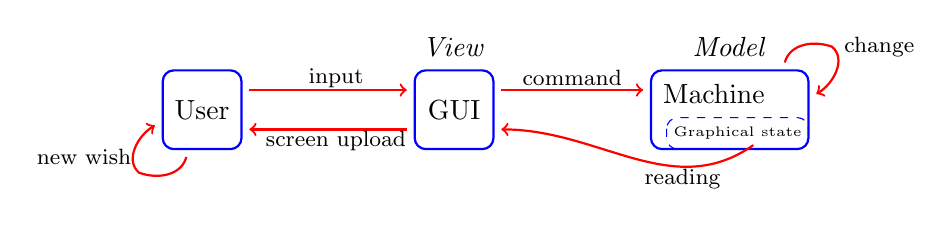
\begin{tikzpicture}

    \coordinate (UU) at (-0.2, 0);
    \coordinate (UC) at (0.3, -0.5);
    \coordinate (UD) at (0.8, -1);

    \coordinate (GU) at (3, 0);
    \coordinate (GC) at (3.5, -0.5);
    \coordinate (GD) at (4, -1);

    \coordinate (MU) at (6, 0);
    \coordinate (MC) at (6.8, -0.3);
    \coordinate (MD) at (8, -1);

    \coordinate (UGS) at (0.9, -0.25);
    \coordinate (UGT) at (2.9, -0.25);

    \coordinate (GUS) at (2.9, -0.75);
    \coordinate (GUT) at (0.9, -0.75);

    \coordinate (GMS) at (4.1, -0.25);
    \coordinate (GMT) at (5.9, -0.25);

    \coordinate (MGS) at (7.3, -0.95);
    \coordinate (MGT) at (4.1, -0.75);

    \coordinate (MMS) at (7.7, 0.1);
    \coordinate (MMC) at (8.3, 0.3);
    \coordinate (MMT) at (8.1, -0.3);

    \coordinate (UUS) at (0.1, -1.1);
    \coordinate (UUC) at (-0.5, -1.3);
    \coordinate (UUT) at (-0.3, -0.7);

    \draw[blue, thick, rounded corners] (UU) rectangle (UD);
    \draw[blue, thick, rounded corners] (GU) rectangle (GD);
    \draw[blue, thick, rounded corners] (MU) rectangle (MD);
    \draw[blue, dashed, rounded corners] (6.2, -0.6) rectangle (MD);

    \draw[red, thick, ->] (UGS) -- (UGT);
    \draw[red, thick, ->] (GUS) -- (GUT);

    \draw[red, thick, ->] (GMS) -- (GMT);
    \draw[red, thick, ->] (MGS) to[out=215, in=0] (MGT);

    \draw[red, thick, ->] (MMS) to[out=75, in=160] (MMC) to[out=320, in=30] (MMT);
    \draw[red, thick, ->] (UUS) to[out=255, in=340] (UUC) to[out=140, in=210]
    (UUT);

    \node at (2, -0.1) {\footnotesize{input}};
    \node at (2, -0.9) {\footnotesize{screen upload}};

    \node at (5, -0.1) {\footnotesize{command}};
    \node at (6.4, -1.38) {\footnotesize{reading}};

    \node at (8.9, 0.3) {\footnotesize{change}};
    \node at (-1.2, -1.1) {\footnotesize{new wish}};

    \node at (UC) {User};
    \node at (GC) {GUI};
    \node at (MC) {Machine};
    \node at (7.1, -0.8) {\tiny{Graphical state}};

    \coordinate (GT) at (3.5, 0.3);
    \coordinate (MT) at (7, 0.3);

    \node at (GT) {\textit{View}};
    \node at (MT) {\textit{Model}};

  \end{tikzpicture}

\end{center}

\caption{Architectural comparision between \emph{Emacs} and \fav.}
\label{fig:archs}
\end{figure*}

The diagram \ref{fig:archs} depicts concisely the way \textit{Emacs}
varies from \fav, almost from the point of view of a programmer. In
\textit{Emacs}, the programmer doesn't really think he programs under or over a
machine. The contents of the machine is exclusive responsability of
\textit{Emacs}, and the interaction or update of it, of the \textit{elisp}
interpreter. But in \fav the programmer have neccesarily to interact with this
machine, since he needs to draw it in a suitable way. This picture tries to
focus on the \textit{Emacs} machine is more like a black box, and in \fav it is
more like a white box, where the programmer need to know things about what is
happening inside it. The ``graphical state'' showed in this diagram tries also
to explain that the machine has an internal structure known for the programmer,
with a special field or part maintaining the actual state of the screen. This
part of the machine is updated each time a graphical routine is executed, and it
says exactly what \fav must exactly show. This point (the black and white boxes
dilemma) is very important, and transports us to the following group of
questions: how does this machine look like? how does the programmer interact
with that machine? Isn't this too heavy?

\subsection{The node concept: machine model}
The central concept or first step of execution of any interpreted language is to
parse the expression the programmer wants to execute. This expression becomes a
syntax tree, and the resulting computation depends completely on this syntax
tree. So, the concept of ``tree'' plays the central rol of any interpreted
language. In \fav, the syntax tree has been generalized to represent the machine
itself. Now, the ``syntax tree'' is only a subtree of the ``machine tree''. We
can simply call it, the \textit{code subtree}. The rest of the tree would
represents the symbol table, the stack of temporary values, the ``program
counter'', the graphical information and any other information \fav needs. The
concrete structure of this ``machine tree'' will be explain further on, in
section \ref{sec:fauppimpl}. The purpose of this section is actually to explain
the concrete rol the ``node'' concept plays in \fav and, above all, why the
syntax tree has been generalized to represent the machine itself.

Paraphrasing the last section, the programmer must and need to think he is
working with a machine, and this makes the contents of the machine very relevant
to him. If before we had two languages with some sort of communication between
them, we need now only one language with high capabilities of introspection,
where the programmer can get new information about the machine over which its
user code is executed. So, it is trivial the machine should have a comfortable
and easily understandable architecture to work with. For this reason,
representing all like a tree is the best way to simplify the machine, for the
following reasons:

\begin{itemize}
\item Since we need at least a syntax tree, this is our lower bound.
\item It is complex enough to represents the information we need.
\item A tree is a structure very easy to explore and to search information on it.
\item It is very scalable: with a new child, you has a new independent subtree
  for adding information. If we want to enrich the machine, adding new child for
  some suitable node is enough, and the rest of the tree doesn't need to be
  changed.
\item It is a universal and well-known data structure. Any programmer with a
  little experience becomes easily familiar with the machine.
\end{itemize}

Lastly, the fact that in \fav all is a node, facilitates optimization, because
only putting efforts to optimizate the implementation of nodes, is optimized
virtually the whole application. In this point it is very important to say how
\fav works: it executes step by step user code in a very granulate way, so
between two uploads or changes of the tree has been executed only a little step
of real code. For example, if the actual step is an assignement, the interpreter
only have to make a little movement of a node: the node representing the rvalue
object, which have to substitute the actual node the lvalue has. This movement
is in fact an operation implemented in the node class. The interpreted have only
to see what is the actual state, and to call the suitable node operations. So,
all computation power is delegated to node operations, and these operations are
consequently our targets for optimizations. The second set of work \fav performs
is the drawing of the screen, and this implies to read the subtree having
graphic information, and to call the suitable \textit{Qt} operations, which
performs the drawing and management of graphical information. But \textit{Qt} is
outside of our control and we can be sure \textit{Qt} is very optimized for
offering these services. In short, the behaviour that we can control is actually
very centralized and therefore easy to optimize.

\subsection{Animating algorithms}
This section tries to answer the question: how do ``animations'' interact with
``algorithms''? or translated to a more concrete question: how does the
``language'' interact with ``the machine''? It is fair to say this question is
not completely solved yet; or better said, its solution is not completely
designed yet, because the language is not completely implemented and I've not
yet experience about how the language works in practice, but I have already any
clear points (advice: since how is the machine implemented has been not yet said
\---that will come in section \ref{sec:fauppimpl}\---, perhaps this section
could be not perfectly understood):

\begin{itemize}
\item As I have already advanced in the previous section, the interpreter works
  in a very granulated way, in the sense the interpreter doesn't perform
  sentences or expressions of user code in one step, but in a sequence of
  uploads of the machine with little modifications. The reason why the
  interpreter doesn't make ``big'' steps to run faster user code is because the
  bigger are these, the less control about the execution process the programmer
  has, and this control its important since the designer could want to animate
  in a very detailed way what is happening in the machine, to animate very
  concrete things like interchanges or simple arithmetical operations (for
  example, to create animations for new computer students who are learning
  programming for the first time), or even, to animate how the machine itself
  works, with ``autodocumentation'' purposes.
\item Since all is a node, all object, syntactic element and variable are also
  nodes. So, the access to the machine itself from the language will be
  implemented by means of a special variable pointing to the root of the
  machine, being the machine a \faupp object like any other. Exploring the
  machine implies only to use this special variable.
\item The language have to offer a way to make ``queries'' to this special
  object (the variable representing the machine) if you don't want to explore it
  completely. If you want to draw something depending on the value of a common
  variable, you wouldn't need to make ``queries'' to the machine; using that
  variable is enough, and you don't need to think you are working with a
  machine. But if you want to detect when a specific instruction is reached, or
  a specific function is called, then you really need any more powerful
  mechanism to make queries.
\item A first type of queries will be the one related to read the ``next'' step
  of execution. For that we need only another special variable pointing to the
  top of the ``program stack''. Reading this variable you know what is the next
  instruction. We can see all our problems can be solved with a new node
  (variable) pointing to another one, or as David Wheeler states: ``all problems
  in computer science can be solved by another level of indirection'';
  translated to \fav: ``all problems in \fav can be solved by another node''.
\item A second type (perhaps innecessary, I have to test that) are those related
  with ``searching'' in the tree. The language could add to its syntax a special
  type of regular expressions which ``should match'' with the state of the
  machine, also returning the involved (matched) nodes. For example, a search of
  this type could be expressed with a sentence like this: ``a node called $x$
  which father calls $p$ and has a depth of 5'', or ``the top of the program
  stack must be termed $assignement$, and there must be another $assignement$
  before, and the rvalue of the first assignement and the lvalue of the second
  assignment must be the same'', for example, to detect any exchange of
  variables.
\item Another way to interact with the ``machine'' is by means of events:
  instead of reading directly the state of the machine, it can be added a new
  event saying: ``call me each time this predicate is true''. This is really the
  best approach for adding automatic animations for specific instructions or
  algorithms.
\end{itemize}

But as I have said before, this will be better defined in the future. The key
issue here is that, this is possible!, thanks to this simplifications, by means
of reducing all to nodes.

Other important aspect to be remarked here is how important the optimization of
the node operations are. Since the interpreter have to work with tiny or very
granulated steps, this ``lost'' of time have to be compensed with very fast
nodes, from their constructions and destruction to its movements, modifications
and any other operations.

How is it designed a common or normal session of \fav? This is a easy question:
like the vast majority of interpreted languages, when \fav runs, the first thing
it makes is to read a start-up file. This file say to \fav the first actions the
interpreter have to perfom, and these actions could be a little menu that, after
clicking in any point of it, loads for you a specific algorithm with its
corresponding animations or views, or any other thing you can program with
\faupp.

A last reflection: why don't work by means of a closer relation between
algorithm and animation, breaking all concepts and designs made so far, in order
to search another simpler way to act, instead of reading and searching on the
machine? There are any good reasons for that, all of them refered to separation
of concerns: in one side, the algorithm shouldn't be polluted with any type of
variables or syntax marks to pass anyhow information to the animations, because
this reduce readability. In another side, a same algorithm could have different
animations or ``views'', so, it's impossible for an algorithm to anticipate
which type of information could need all of its animations. A third problem is
the programmer of an algorithm could be completely independent persons. So, for
a same algorithm different animations could be implemented, for different
persons, and in differents moments, each time with different needs (for
explaining different aspects, for example), purposes (for offering more complex
or detailed views) or simply style (different teachers could have different ways
to explain the same thing, and different students could need different ways to
understand a same algorithm). So, keeping independent animations and algorithms
is a positive solution for each possible objection, and also it brings the
adventage of designing easier a database of algorithms and animations and of
allowing final users to select the algorithms with the views they want.

\section{Language features}
Before going to the next step, lets me repeat the chain of problems and
arguments which have brought us to here. First and foremost, the first target is
allowing the user to write algorithms and develop animations for them. The first
conclusion was if you want to have a flexible enough way to develop animations,
you need a programming language, having thus two: the language for writing
algorithms with its corresponding interpreter, and another language for writing
animations, with again its corresponding interpreter. But, if we have two
languages, why not having only one? If not, it would be neccesary to design,
develop and maintain two languages and interpreters. What was before
communication between two languages, is now a language with high capabilities of
introspection, for getting information of itself in execution time. So, the next
focus was the machine itself. The machine should be a simple structure, to
facilitate the getting of information. Since we need at least a syntax tree, in
order to don't create a most complex one, the syntax tree was generalized for
representing the whole machine. So, the node concept is now the central aspect
to focus on. It has the disadventage of forcing the interpreted to do little
steps to facilitate an explicit or easier control about what is happening in the
machine, but alsp the adventage to make \fav easily optimizable, because all
behaviour of \fav becomes operations on nodes. So, animating algorithms is not
more than writing algorithms and animations in a separate way, the second one
reading the state of the machine to get information about the state of
computation of the first one, and the first one being executed only when the
final user asks somehow for it. Lastly, the machine could be implement with no
more than a common variable of the language, since in \fav all objects are
implemented as nodes, with the machine itself being another one (the root
actually).

The next step is, finally, to design how the language really is and how
developers can program something for \fav and which features it has. The target
of my design was always simplify the ``model memory'' or the ``behaviour'' of
the language machine, even though sacrifying the possibility to design a
language with a simple syntax. Anyway, the ``syntax complexity'' can be always
simplify be means of syntactic sugar for make easier or comfortable the most
common or required actions or expressions. The purpose of this section is to
show the elements of the language, together with its syntax.

It is fair to say also that the language is not completely implemented. In fact,
its implementation is in its first steps, so the working examples I can provide
are minimal.

% too hard? simplifying algorithms. Advertise about the language is in its first
% steps. The logical order is, first language, and after implementation, but the
% real one was ``intercalado''.

\subsection{Sources of inspiration}
In this section will be discussed features of \faupp focusing on how I have
reached these conclusions and which reasonings there are behind them. After this
section, I will speak about the language focusing in the language itself. The
way I have made decisions was based on my experience with different languages,
its good and not so good points, and also on new languages that I've discovered
while I was searching solutions for my design.

\subsubsection{\textit{C++} and \textit{Octave}}
One of my first ideas about the features of \faupp was those related to the type
system. I had clear even from the beginning the system will have types, but my
doubts was related to if the type system would be static and strong (like
\textit{C++}, which requires the type of each object must be known in
compilation time) or dynamic and weak (like \textit{Octave}, which computes the
type of each object when objects are created and without indications about what
types can accept each variable). In one side, a function without type marks
(like \textit{Octave}) has a more mathematical aspect. But in the other side,
types improve security for the programmer, at the same time it becomes more
troublesome and decrease readability. For example, in my experience with
\textit{Octave}, I've verified by myself with the ease with which you can get an
error in a very different point of the one where the real error happened, only
because you have send an object to a function, with a different but compatible
structure and defined operations than the function expected to receive,
returning thus some inconsistent value, which survives a few additional lines of
code until you notice some error did happen, only because that value ``worked''
in a syntactic point of view. For this reason, my functions in Octave had always
the same structure: a kind of header with different lines checking types and the
rest of the function the lines with the real implementation.

The type system of \faupp, or better said, its ``type marking'', selects an
intermediate point between these two ends of the string: functions in \faupp
have typed input and output parameters, but local variables are without type
marks. In my view, this is a very good solution, because a developer knows what
he are doing and he doesn't need all the verbosity of strongly types languages
for programming the behaviour of its function, above all because a function is
usually programmed by a single person, but it can be virtually used by
anybody. So, the security efforts are focused on function interfaces, adding
``mandatory'' type marks to its parameters (inputs and output) and allowing more
flexibility in function bodies. With that, we have earned the adventage of
making easy to developers to write new functions, and also the adventage of
improving security avoiding other developers use them accidentally wrong,
exactly the adventages of both languages together, and without their
disadventages.

\subsubsection{\textit{C++} and \textit{elisp}}
Other question was about ``name scoping''. Since I work fundamentally with
\textit{C++}, this is always my first reference when I'm designing another
feature of my language, even though my conclusions turn away from
\textit{C++}. There are essentially two different types of ``name scoping'',
represented here for \textit{C++}, our first reference, and \textit{elisp}, our
counterexample:

\begin{itemize}
\item In \textit{C++}, local variables obscure global variables if there's a
  conflict of names and there is no ways to create new global variables from
  local scopes. All new variable declared inside a local scope, has that scope.
\item In \textit{elisp}, however, the command \texttt{setq} creates, or changes
  if it already exists, a value for a global variable. The other way to create
  variables is with the command \texttt{let}, which creates variables of
  expression scope, and there is really no ways to declare local scope
  variables. The only way to simulate this effect is by means of a \texttt{let}
  command at the very beginning of the function definition. In \textit{elisp},
  moreover, there is no restrictions about when new names can appear. If a body
  function uses a non-declared name in its points of definition, there is no
  problem, because the only restriction is the name exists when this function
  is called, and not when is defined, as it happens in \textit{C++}.
\end{itemize}

Although all dynamic behaviour is more comfortable, it has also new problems
regarding security, because the possibility of name conflicts
increases. \textit{Emacs} source code has an high tendence to create variables
with more prefixes and ways to avoid conflicts with other names. If \textit{C++}
has inserted the ``namespace scope'' on top of its block and local scopes, is
precisely for that reason: avoiding conflicts to increase security.

In \faupp, again, we have choosen an intermediate solution between these two
extrems. In \faupp, it exists local and block scopes, but nor expression scope,
neither ways to create new global variables from local scopes (or not at the
moment), like in \textit{C++}. Each function or block has its exclusive scope
(together with its inherited scopes), but the name policy works as
\textit{elisp}, where body functions are not checked for name existence and the
only requirement is names exists when they are needed. So, in \faupp, you can
use variables inside new definitions even if they don't yet exists.

The restriction of using already defined variables, like in \textit{C++}, is
called lexical scope, because names are checked at the very moment the compiler,
which reads the file in a lexical order, found them, and the way
\textit{lisp}, \textit{elisp} and other \textit{lisp} dialects and interpreted
languages work, is called \textit{dynamic scope}, because names are searched and
found in execution time. So, if I should define in which category \faupp belongs
to, I will say it belongs to a dynamic scope one, but not completely, for the
following reason: a language implementing pure dynamic scope has normally only
one symbol table, corresponding to the global scope, and each symbol is really a
stack of values. Each time a new local variable is created, a new value is
pushed in its corresponding stack (if the name already exists, if not, a new
variable/stack is created), and each time this scope ends, each new created
variable is popped. \faupp, however, doesn't work on this way and it uses true
symbol tables for each scope, because the nature of \faupp scopes and objects
facilitates this way of working (see section \ref{ssec:object}). So, \faupp has
dynamic scope with features of static scope.

Why have I choosen this way of proceeding? For optimization reasons. If \faupp
doesn't check that each variable is previously defined, is because this checking
consumes time, especially when the number of user code grows. If it wasn't for
optimization reasons, \faupp will be static typed, because it is more sure.

\subsubsection{The \textit{Axiom} algebra computer system}
Since it was decided \faupp is an object-oriented language, to enjoy the
adventages that object-oriented languages have for developing big programs, the
interpreter must manage at least the following aspects: type checking,
function definitions, class or object structure, inheritance, anonymous or
temporary objects, symbol table, name mangling and scopes, function
polymorphism, the different statements, and expressions.

I was searching a way to reduce this list to the tiniest one, unifiying the
maximum number of possible concepts. This preocupation is related to the machine
itself: the simplest are the concepts with which the interpreted have to work,
the simplest are the machine itself, and thus, the most comfortable is the way
developers can interact with the machine.

A source of inspiration to found a way to reduce this list was the
\textit{Axiom} system. The \textit{Axiom} system is an algebra computer system,
and its behaviour is thus oriented to the operations which are defined for each
type. So, Axiom forces you to think, when you create a new type, which
operations this type will have, and not which structure. And remembering our
discussion about the type system, we reached to the conclusion that forcing
functions to type its interface (inputs and output) is the best way to improve
security. But, exactly, for which reason? I mean, what is more important to a
function, knowing the structure of its inputs, or knowing the available
operations together with its properties of its inputs? In my experience and
opinion I should say, for the function itself is more important the available
``behaviour'' of its input parameters (how the functions can use its inputs) but
for other functions using the first one, it is more important the structure of
the returned values, because a function, in a external point of view (the used
function), implements behaviour, but in an internal point of view (the function
itself), operates with data. So, the debate is opened, and the rol the
\textit{Axiom} system has played in my reasonings about the features of \faupp,
was precisely to see this difference is important.

The way \textit{Axiom} implements this behaviour, is similar to the use of
\textit{Java} interfaces, or \textit{C++} abstract classes, with a little rename
of names. In \textit{Axiom}, ``interfaces'' are called ``categories'', and
``types'' are called ``domains'' (of computation). In \textit{Axiom}, categories
declare operations and also constants, like 0 or 1 (\textit{Axiom} says,
categories export \textit{symbols}, making reference to any declared identifier,
either function or constant), while domains implements categories by means of
adding a data structure, and defining the declared symbols. Like \textit{C++}
and unlike \textit{Java}, in \textit{Axiom} is possible that categories
(interfaces/abstract classes) implement any operation it wants if you don't need
an implementation for that, for example, using other operations of the same
category (of course, is a natural consequence of not having a data structure
that almost one operation remains without definition). The most trivial example:
the operator \texttt{!=} can be defined negating \texttt{==}, and derived
domains only would need to implement the operator \texttt{==}. The way
\textit{Axiom} promotes the use of categories is defining a big tree of
predefined categories, for example, a so simple domain like \texttt{Integer}
inherits \texttt{IntegerDomainSystem}, who declares, among others, the
\texttt{add} and \texttt{random} operators, and the symbol \texttt{Infinite},
the only one with which \texttt{nextItem} returns the same value. At the same
time, \texttt{IntegerDomainSystem} inherits from other 14 categories like
\texttt{EuclideanDomain}, \texttt{DifferentialRing} or
\texttt{CombinatorialFunctionCategory}, which ultimatly inherit from
\texttt{SetCategory}, via other categories like \texttt{OrderedRing},
\texttt{Monoid}, \texttt{Algebra}, \texttt{Ring} or \texttt{AbelianGroup}. The
other aspect \textit{Axiom} try to focus is the properties of these operations
must have, because properties are fundamental aspects of algebraic
structures. Since \textit{Axiom} is not a pure funcional language and since it
is imposible for a computer to proof a property is true (it is a no-computable
problem), \textit{Axiom} provides no syntactic ways to specify these properties
(except comments), and developers of new categories or domains have the
responsability to ensure their new domains or categories have the same
properties as the categories they try to inherit.

Although \faupp doesn't implement explicitly in its grammar a distinction
between category and domain, it does also focus on this way of describing or
dealing with types, because it is more mathematical, and the mathematical way
is, in my opinion, a more didactic and comprensible way of presenting
algorithms, since algorithms with educational purposes does usually solve
problems of abstract structures like graphs, vectors, different types of trees,
hash tables or even solving pure analytic problems, like those of
cryptography. Moreover, if \faupp focus on that way of ordering or
relating types, \textit{developers} will create new types more carefully, trying
to reuse definitions, and ultimately facilitating algorithm categorization,
according to the types over they work.

\subsubsection{Prototype-based languages}
Prototype-based languages are languages where there is no clear distinction
between ``type'' and ``object''. Examples of these languages are
\textit{Javascript}, \textit{Self} or \textit{ECMAScript}. Objects are created
in this kind of languages in a ``in-line'' fashion: structure of objects are
specifying with a ``dictionary-like notation'' where you can specify fields and
contents of your new objects, and inheritance is expressed by means of a special
type of composition, so, there is no syntactic way to think about classes: all
are objects. In the following snippet, a little example with a ``fictitious''
syntax representing real protype-languages is showed and explained:

\begin{Python}
  person <- {name: "Aaron", surname: "Bueno", age: 25}

  student <- {field: "Computer science"}

  student.#base <- person

  print("%s ", student.name, "%s ", student.surname, "%d ", student.age,
        "%s", student.field)
\end{Python}

In this case, a object \texttt{person} is created from scratch and it doesn't
represent any real type. Its fields are name, surname and age, expressed in a
dictionary way, like those of \textit{Python}. \texttt{Student} is another
object, and in the third line, the object \texttt{student} ``inherits'' from
\texttt{person} in a very dynamic way. These objects are cloned, so,
\texttt{student} can modify is ``own'' copy of \texttt{person}. This kind of
languages have always a special syntax to distinguish between common composition
and inheritance (like \texttt{\#base}). The difference among composition and
inheritance lies in that inheritance merges the interface of the base object
with its derivated object, and common compositions doesn't. The second
difference is a object which inherits from other object is saying: ``I'm a
concrete instance of my base, and I can substitute it anywhere it is
accepted''. For this reason, it is important to maintain a special way of
indicate this \textit{special} type of composition.

This behaviour or way of acting go very well with our purpose of symplifying
\faupp, and the number of concepts are reduced, because class or type definition
and inheritance are merged with composition, by means of a special kind of
syntax, and also increasing possibilities of dynamic behaviour.

\subsubsection{String-based languages}
Other sources of insipiration were the language \textit{bash}, a programming
language, and above all command processor, favourite son of \textit{Unix}
systems, and \textit{CMake}, a build system to facilitate the compilation
process in a cross-platform way and also an alternative tool to other system
like \textit{autotools} or \textit{qmake}. Both of them, \textit{bash} and
\textit{CMake}, have as primary data type ``strings'', and all operations are
performed over strings, being arithmetical operations a secondary target.

Other inspirating language was \textit{Thue}. It is considered an ``esoteric''
programming language, but it does also have interesant characteristics that
could be added somehow in \faupp. The \textit{Thue} system is a
\textit{rewriting system} (and a non-deterministic language) which is based on
semi-Thue grammars and it implemets in a very direct way type-0 grammars
(unrestricted grammars) of the Chomsky hierarchy, and thus, it is a
Turing-complete language\footnote{Although the main site of the \textit{Thue
    programming language} says that it is \textbf{believed} to be
  Turing-complete, but \textit{semi-Thue systems}, the formalism which
  \textit{Thus} is based on, are in fact demonstrated to be Turing-complete.}.

The behaviour of \textit{Thue} will be explained by means of an example, extracted
from the the wikipedia article about the \textit{Thue} system:

\begin{Thue}
  b::=~0
  b::=~1
  ac::=abc

  ::=

  abc
\end{Thue}

This code will transform the entry \texttt{abc} by a random sequence of
\texttt{0} and \texttt{1}. The procedure is as follows:

\newcommand{\mathred}[1]{\textcolor{red}{#1}}

\begin{center}
\begin{tabular}{lcrcrr}
  \textit{Input} & & \textit{Match} &  & \textit{Output} & \textit{Rule} \\
  \hline
  $abc$ & $\Rightarrow$ & $a\mathred{b}c$ & $\Rightarrow$ &       & $(1, \mathred{2})$ \\
        &               & $\mathred{ac}$  & $\Rightarrow$ & $1$   & $(\mathred{3})$    \\
        &               & $a\mathred{b}c$ & $\Rightarrow$ & $1$   & $(1, \mathred{2})$ \\
        &               & $\mathred{ac}$  & $\Rightarrow$ & $11$  & $(\mathred{3})$   \\
        &               & $a\mathred{b}c$ & $\Rightarrow$ & $11$  & $(\mathred{1}, 2)$ \\
        &               & $\mathred{ac}$  & $\Rightarrow$ & $110$ & $(\mathred{3})$   \\
        &               & $a\mathred{b}c$ & $\Rightarrow$ & $110$  & $(1, \mathred{2})$ \\
        &               & $\mathred{ac}$  & $\Rightarrow$ & $1101$ & $(\mathred{3})$   \\
\end{tabular}
\end{center}

In the code, the fifth line distinguishes between definitions and inputs from
the program. So, the input is \texttt{abc}. From this input, \textit{Thue}
searches a match among its productions rules, extracting the matched expression
from the input. It founds the productions $1$ and $2$ and \texttt{b} is
extracted from the input, which becomes \texttt{ab}. \textit{Thue} selects one
of the found productions randomly. For example, the second one is selected. The
right side of this production is always a ``replacement'', except if the symbol
\texttt{\~} is found, which means to put something in the output. In this case,
the number \texttt{1} is sended to the output. Our new input \texttt{ac} match
with the third production rule, and our new input is its replacement:
\texttt{abc}. The operation is repeated: it is found two replacements for
\texttt{b}, and the second production rule is again selected, sending another
\texttt{1} and replacing nothing. Our output is now \texttt{11} and we have no
replacement for \texttt{b}. So, our input is actually again \texttt{ac}. In a
recursive way, the system replaces the next \texttt{b} by 0, after by 1 and so
on, selecting randomly one of the founded productions and consequently getting a
randomly sequence of 1 and 0.

Since rewriting system are Turing-complete, and what a developer writes in a
source file are strings (things typed from his keyboards), focusing \faupp as a
more string-oriented language is not a bad idea at all. Not in the way
\textit{bash} and \textit{CMake} works, because their behaviours are more
adequate for other purposes, but more oriented to allow developers to create its
own basic types based on regular expressions, and erasing primitive and
pre-implemented types like numbers or booleans, managing only strings. This
thing could be very comfortable and a way to personalize and extend the grammar
of \faupp. This could be achieved using these regular expressions to define
lexical descriptions of new types, and rewriting rules like those of
\textit{Thue} to implement the most basic operations. In fact, \faupp already
use (internally) some mechanism based on regular expressions, to experiment with
them, to see how far feasible this behaviour is in optimization terms.

In the next code snippet, it is showed a possible implementation of a manually
created definition of a basic type like \texttt{PositiveInteger}, together with
its function \texttt{next}, to illustrate rewriting system can be really useful
and not necesarily verbose:

\begin{Thue2}
PositiveInteger ::= [0-9]+

PositiveInteger next(PositiveInteger v)
{
  rewrite(v, w) {
           . ::= _.  // (0)
          0_ ::= 1   // (1)
          1_ ::= 2   // (2)
          2_ ::= 3   // (3)
          3_ ::= 4   // (4)
          4_ ::= 5   // (5)
          5_ ::= 6   // (6)
          6_ ::= 7   // (7)
          7_ ::= 8   // (8)
          8_ ::= 9   // (9)
          9_ ::= _0  // (10)
          _0 ::= 10  // (11)
  }

  return w;

}
\end{Thue2}

In that code, it is define that any expression written as a sequence of symbols
from 0 to 9 is a \texttt{PositiveInteger}, and a function \texttt{next}, defined
over \texttt{PositiveInteger}s. This function would receive a
\texttt{PositiveInteger} \texttt{v}, and the output would be computed by means
of the statement \texttt{rewrite}, which is an embedded rewriting system working
like \textit{Thue}, and the results being saved in \texttt{w}. From a number
like \texttt{2399}, with its implicit character \texttt{.} signaling the end of
the expression (\texttt{\$} in other languages), this rewriting system would
perform the following transformation:

\begin{center}
\begin{tabular}{ccrr}
2399. & $\Rightarrow$ & 2399\mathred{.}   & (0) \\
      &             & 239\mathred{9\_}.  & (10) \\
      &             & 23\mathred{9\_}0.  & (10) \\
      &             & 2\mathred{3\_}00.  &  (4) \\
      &             & 2400.             &
\end{tabular}
\end{center}

The last production is useful for strings like \texttt{99}, where the character
\texttt{.} is transported from the beginning of the expression to the end:

\begin{center}
\begin{tabular}{ccrr}
99. & $\Rightarrow$ & 99\mathred{.}    & (0) \\
    &               & 9\mathred{9\_}.  & (10) \\
    &               & \mathred{9\_}0.  & (10) \\
    &               & \mathred{\_0}0.  & (11) \\
    &               & 100.
\end{tabular}
\end{center}

So, we can see this could be a good and comfortable way for allowing users to
write its own ``syntax'' from special situations were they could be useful, and
to extend the language with new constructions without having to change \faupp
itself, for example to add support to express in a comfortable way complex
things like Turing machines or expressions of lambda calculus.

\subsection{The object concept}
\label{ssec:object}
Since \faupp is an object-oriented language, the first and principal concept
that can be defined is how are objects. Objects in \faupp are a very compact
structure grouping structure, function, type, and polymorphism (subtype and
parametric polymorphism).

Before contuining, it is assumed the reader knows and domains object-oriented
languages and their concepts and common behaviour.

A \faupp object is a callable entity, and in this sense it behaves like a
function. An object consists in two parts:

\begin{description}
  \item[Context] A grouping of data, with information about its composed and
    inherited objects, which life is the same the life the object itself. It is
    in fact a ``function closure'', that means, a ``reference environment'',
    that exists each time its functions is called, in this case, that exists
    each time the object is called. The context keeps the objects it is composed
    of and also its base objects. The context implements, at the same time, the
    ``type'' or structure of the object, and subtype polymorphism. Also,
    contexts work like symbol tables and controls the scope. All executable
    entity has its context loaded, and there is no executable entity which is
    not an object. If new variables are created, they are saved in the context
    of the most recent object being executed. The start-up file, which represent
    the main function of common programming languages, is also an object itself.
  \item[Overloads] An object doesn't represent a ``function'' but a grouping of
    function related semantically, or, better said, a callable entity computing
    somehow the same thing, with independence of the way this callable entity
    (this object) is called. In a more concrete way, with independence of its
    parameters: if some functions are somehow very semantically related, can (or
    should) be implemented like differents overloads of the same object. The
    first adventage is the context is shared for all of its overloads. The
    ``overloads'' section does thus implement at the same time, behaviour and
    parametric polymorphism.
\end{description}

Finally, a object can be named or unnamed (anonymous):

\begin{description}
  \item[Named object] A named object represents a variable. If an object is named,
    it has a persistent lifetime (also called, \textit{extent}).
  \item[Anonymous object] Objects created ``in-line'' inside expressions. The
    most typical anonymous object are returned ones by other objects after. It
    has the same lifetime as the expression that contains it.
\end{description}

Before continuing, lets me present how objects must be used and how names
work.

\subsubsection{Object names and utilization}
What assignments does really make in \faupp is to name anonymous objects. In a
expression like this:

\begin{faupp2}
  a <- <expr>;
\end{faupp2}

the right side of the assignment creates an unnamed object, and the left side of
the assignment names this object with the name \texttt{a}. So, from this time,
each time I write any other expression that contains \texttt{a}, I'm calling
this object returned by the expression.

\begin{faupp2}
  a <- <expr>;
  a;
\end{faupp2}

After assigning \texttt{a}, \texttt{a} is a named object, and since objects are
callable entities, writting its name implies call it, and thus, executes some
overload. In this case, without parameters, and if there is an available
overload without parameters (with an empty list of parameters), this overload is
called. The overload without parameters is call in \faupp the \textit{default
  overload}. As constructors in \textit{C++}, if there is any explicit overload,
a default overload is always provided. This \textit{implicit default overload}
does always return a copy of itself.

More concisely: objects has by default an implicit default overload, returning a
copy of itself (simulating common variables of common programming languages),
but if it has one explicit overload (written by a developer), the implicit
default overload is erased. At this point, if the object has a default overload
or not (the overload without parameters) is responsability of the developer.

Moreover, \faupp is a very economic language, and it pretends to save you
writing. So, since each object in \faupp is a callable entity and the only
thing you can make with it is call it, if you want to call the default overload
of the object, you don't need to write an empty list of arguments between
brackets. Writing the name of the object is enough. This type of saving will be
seen again in different points of this report.

\begin{faupp2}
  a;    // Default overload of 'a' called.
  a();  // Equivalent expression.
\end{faupp2}

In the two previous sentences, if \texttt{a} has no explicit overloads: its
execution returns a copy of itself. If \texttt{a} would have explicit overloads,
but not a default one, an error would be reported in the first line.

The following snippet makes evident the fact only there can be one object with
the same name at the same time, or more concisely, if we think a name as an
entity ``pointing'' to an object, if a new object is named with an already
existent name, this name changes its ``pointer'' to the new object, and the old
object ends its lifetime.

\begin{faupp2}
  a <- <expr>;
  a <- <another_expr>;
\end{faupp2}

Currently, there is also no ways to create two different names for the same
object. In a code like this:

\begin{faupp2}
  a <- <expr>;
  b <- a;
\end{faupp2}

the new name \texttt{b} names an anonymous object, exactly that returned after
calling the default overload of \texttt{a} (reminder: the \textit{default
  overload} is the overload without parameters, irrespective of if this overload
is implicit or explicit, and the \textit{implicit default overload} is the one
which returns a copy of itself if there is no explicit overloads).

\subsubsection{Creating new objects}
The most basic expression you can write in \faupp is a new object. Its (reduced)
syntax is as follow (exemplified inside an assignement):

\begin{faupp2}
  a <- [ <stmnts> ]
       : <type_mark> ( <params> )
         { <stmnts> }
       : <type_mark> ( <params> )
         { <stmnts> }
       // more overloads
       ;
\end{faupp2}

This manual and direct way to define objects is called an \textit{inline
  definition}.

As advice, names between angles brackets (\texttt{<>}) used throughout this
report does not exactly or not always correspond with names used in the grammar
of \faupp, and the names presented here has been renamed for undertability
purposes. For example, the non-terminals representing a sequence of
statements is called in the \faupp grammar, \texttt{<seq>}, but
\texttt{<type\_mark>}, \texttt{<return\_mark>}, and \texttt{<stmnts>} (statements)
and \texttt{<type\_mark>} are more intuitives.

If an overload is indeed a procedure and not a function, you can omit the
\texttt{<type\_mark>}. If you are writting an explicit default overload, which
has a empty list of parameters, you can also omit its (empty) brackets. If an
object has an empty context, you can omit also the square brackets. Even more,
if a default overload is at the same time a procedure, you can omit also the
colon, writting only the list of statements implementing the overload, together
with their enclosing braces.

Examples of ``minimal'' objects you can write in \faupp are the followings:

\begin{faupp2}
  a <- [];
  a <- {};
  a <- []{};
  a <- :(<param>) {};
  a <- :<type_mark> {};

  a <- [] :(<param>, <param>)
           {};

  a <- [] :<type_mark>(<param>)
           {}
          :(<param>)
           {};
\end{faupp2}

Two additional observations. The first one is that statements in \faupp are
postfixed by semicolons (\texttt{;}). At the beginning was intented to create
\faupp as a language where line breaks and tabulators control the limits of
statements, and not special characters like \texttt{;}. This is for example the
case of \textit{Python}. But the wanted flexibility for \texttt{faupp} together
with the complexity of the syntax of objects, made this pretension impossible, or
better said, too much verbose, for an automatic grammar generator like
\texttt{bisoncpp}, the automatic grammar generator used by \fav.

For the same reason a statement like:

\begin{faupp2}
  b <- a;
\end{faupp2}

implies to call \texttt{a}, an inline object is also called before the
assignment happens:

\begin{faupp2}
  // 'a' will be the name of the returned
  // object after calling <obj>.
  a <- <obj>;
\end{faupp2}

The correct syntax to name directly an inline object without execution is with
the operator \texttt{\char`\&<-} instead of \texttt{<-}, but this operator is
not implemented yet.

\subsubsection{Calling objects}
Given an object defined as follow:

\begin{faupp2}
  a <- {
         b <- [];
       };
\end{faupp2}

this object is equivalent, as already said, to the following one:

\begin{faupp2}
  a <- [] : ()
       {
         b <- [];
       };
\end{faupp2}

and, as also already said, this inline object is executed before being assigned
to \texttt{a}. What overload is called? the default overload is called, or what
is equivalent:

\begin{faupp2}
  a <- [] : ()
       {
         b <- [];
       }();
\end{faupp2}

This means: given this inline object, it is called its default overload. It's an
equivalent expression to the one presented before. What does it happen after the
execution of this overload? The assignment fail in its attempt to name the
object returned, because this overload is a procedure and nothing is returned,
so, there is no object to be named. If there is no explicit overloads, the
default overload returns a copy of itself:

\begin{faupp2}
  a <- [];
\end{faupp2}

This object has no explicit overloads, and thus, \texttt{a} would be the name of
the returned object by its implicit default overload, which returns a copy of
itself. So, \texttt{a} is currently a named object with an empty context and
only the implicit default overloads:

\begin{faupp2}
  a <- [];
  b <- a;
  c <- b;
\end{faupp2}

In this code, \texttt{a}, \texttt{b} and \texttt{c} have empty object:
\texttt{a} because the reasons given before, \texttt{b} because the object
\texttt{a} is called, and the same process as in the construction of the object
\texttt{a} is repeated: \texttt{a} contains an empty object, this object is
called, returning a copy of itself, which is named \texttt{b}. And lastly, the
same process is repeated and a copy of this empty object is received.

But objects can also be used directly as statements to simulate ``blocks'' of
common imperative languages:

\begin{faupp2}
  {
    b <- []; // (*\label{bnul}*)
  };
\end{faupp2}

In this example, a temporary object is created an executed. In its execution,
the empty object \ref{bnul} is assigned to the object \texttt{b}. But, where?
For answering this, it is neccesary to know how does contexts work.

\subsubsection{Object structure}
\ffaupp works by means of a stack of contexts, which controls the ``name
scoping'' and the ``name resolution'' of \faupp and corresponds to the
\textit{symbol table} in the jargon of common programming languages.

Each time a new object's overload is called, the context of the called object is
pushed in this stack, and it is additionally created an automatic context,
pushed on top of the object's context, representing the local context of the
overload itself. In this context the parameters of the function are saved, as
well as any other local variable created in the overload execution. The context
of the object is thus called the \textit{object context}, and the context of the
overload is called the \textit{local context}.

And what is the first, or ``global'' context? When \fav is opened, the first
thing the interpreter read is a statup-file called provisionaly
\texttt{.faunit}. This file contains a sequence of statements:

\begin{faupp2}
  <stmnt_1>;
  <stmnt_2>;

  // more statements

  <stmnt_n>;
\end{faupp2}

but this sequence is equivalent to an implicit called object:

\begin{faupp2}
  /* implicit [] */
  {
    <stmnt_1>;
    <stmnt_2>;

    // more statements

   <stmnt_n>;
  } /* implicit () */;
\end{faupp2}

and, like any other object, this implicit object has an object context and a
local context. This object is called the \textit{startup object}, its default
overload (the only overload of the startup object), \textit{startup overload} and
its local context, the \textit{startup context}. The object context for this
startup object is omitted, since it is irrelevant, non persistent (the startup
object is besides an anonymous one) and contains no information. In short words,
the startup object is a special object without object context. The lifetime of
the startup object is at the same time the lifetime of a \fav session.

The name lookup procedure of \faupp is expressed by means of the following code
sample:

\begin{faupp2}
  // {
  a <- <expr_1>;

  // implicit []
  {
     b <- <expr_2>;
     a <- b;  (*\label{ab}*)
  };
  // };
\end{faupp2}

In this code, the first statement creates an object \texttt{a} with the output
of executing \texttt{<expr\_1>}. The second object creates two additional
contexts: the object context (empty in this case), and the local context of the
called overload (the default overload in this case).

Within this object, a object \texttt{b} is created with the output of
\texttt{<expr\_2>}, and the next step is executing \texttt{b}, and its output is
named \texttt{a} (line \ref{ab}). The next question is, is it created a new
named object \texttt{a} or the global \texttt{a} is overwritten? And the answer
is: the global \texttt{a} is overwritten. The first thing \faupp makes is to
search the nearest context where the searched name is. If this name is found,
this context is used to put the new object. If this name is not found, the most
nearest context is selected to put the new name. In this case, the nearest
context is the local context of the overload actually being called.

Returning to the example, \texttt{a} is defined in the global scope, and this
will be the scope of the new named object returned in $(1)$. When this overload
finishes its execution, both (local and object) contexts are popped and
consequently, the name \texttt{b} no longer exists, since this object was
temporal.

If the previous examples are carefully readed, the reached conclusion is named
objects are always saved in local contexts. Local variables of overloads are
saved in local contexts, and global variables are in fact local variables of the
\textit{startup context}. But, what contains object contexts and how are they
constructed?

\begin{faupp2}
 a <- [
         <stmnt_1>;
         <stmnt_2>;
         // more statements
         <stmnt_n>;
      ];
\end{faupp2}

Here we have an object which constructions is driven by this sequence of
statementes. When a new inline object is reached, the construction process of it
begins creating a new empty context (the object context), and after it the
statements inside it are executing in the same order, using this object context
as the local context of this sequence (as it happens in overloads). After it,
an overload of it is called: if the developer has specified which overload
should be called, it is created the local context of this call and this overload
is executed, returning as this overload said. If not, the implicit overload (if
it exists) is called. If this implicit overload is the implicit one, it returns
a copy of itself (included the object context). The next time I call this object
(if this object is named, of course), the object context does yet exists and
with the same contents.

This is an important point, because while common object-oriented systems
define the structure of objects by means of a list of variables, optionally with
their default values, in \faupp the structure of this object is the outcome of
the execution of the statements inside the definition of the context.

For example:

\begin{faupp2}
  a <- [
          a <- <expr_1>;
          b <- <expr_2>;
       ];
\end{faupp2}

In this example, \texttt{a} will be the name of a new object with two subobjects
(or also they could be called, \textit{fields}), \texttt{a} and \texttt{b}, whose
values are the returned object by the expressions \texttt{<expr\_1>} and
\texttt{<expr\_2>}.

In terms of other object-oriented languages like \textit{C++}, it is like if
classes have only one possible constructor. But, this doesn't mean the values of
the fields of the context can not depend on parameters? No, it doesn't mean
this, because the construction process can be delegated to the
overloads. Example:

\begin{faupp2}
  my_type <- [
                a <- [];
                b <- [];
             ] { return /* myself */; }
               : ( <param> )
               {
                 ret <- my_type;

                 ret.a <- <expr_1>;
                 ret.b <- <expr_2>;

                 return ret;
               };

   obj <- my_type(<arg>);
\end{faupp2}

In this example, I'm simulating a class constructor. When the inline object is
executed, its default constructor is called, since there is no explicit
call. This default constructor returns a copy of itself. If the word
\texttt{myself} is currently commented is because there is no defined syntactic
expression to refer to \texttt{myself} (as \texttt{self} in \textit{Python} or
\texttt{this} in \textit{C++}).

But, in the second assignment, the second overload is called. This overload
calls \texttt{my\_type}, this returns a copy of \texttt{my\_type}, an object
with two empty fields: \texttt{a} and \texttt{b}, and this new copy is called
\texttt{ret}. The next two lines modify this object \texttt{ret}, assigning
new values to these fields, and in the last step, \texttt{ret} is returned and
called \texttt{obj}. And in passing, the way fields are refered and how objects
are returned are shown.

It exists also a second way to define structures, this can be very
comfortable. It is called the \textit{force operator}:

\begin{faupp2}
  => a.b.c.d
\end{faupp2}

This expression creates in sequence:

\begin{enumerate}
\item An empty object \texttt{a}.
\item The object context of \texttt{a} is enriched with a new empty object
  \texttt{b}.
\item The object \texttt{a.b} is enriched with \texttt{c}.
\item The object \texttt{a.b.c} is enriched with \texttt{d}.
\end{enumerate}

Also, this could be used to create new empty objects, as alternative to other
simple forms:

\begin{faupp2}
  => a; // Equivalent to:
  a <- [];
\end{faupp2}

Of course, I can assign values to this forced objects, or use them inside
overloads or contexts:

\begin{faupp2}
  => a;
  => a.b.c.d <- <expr_1>;
  => a.c;

  o <- [
         => field1;
         => field2;
         => field3 <- <expr_2>;
       ] : {
         => other_obj;
         => another_obj.field <- <expr_3>;
       };
\end{faupp2}

This examples pretend to make manifest although using objects in its more pure
way can be perhaps verbose, with a little of magic syntactic sugar any statement
or ``way of expression'' can be very simplified. The most important thing to be
remarked here is, although syntactic sugar can simplify your writting and also
help you to think in a more superficial way, the internal concept are nor modify
neither affected by the added syntactic sugar.

\subsection{Expressions}
In this section will be exemplified how expressions works in \faupp. In common
languages, there is normally tree types of expressions: constant objects
(numbers, strings), operators, which can be infixed binary operators
(\texttt{+}, \texttt{*}), prefixed unary operators (\texttt{!}, \texttt{\&}),
postfixed operators (\texttt{[]}) or more complex ones (\texttt{?:}), and the
third type of expression are function calls. These third type of expressions
could be seen as a concrete type of postfixed operator (\texttt{()}), as
\textit{C++} does. Other languages use only constant objects and prefixed
operators, like \textit{bash} or \textit{lisp} and its dialects do. In \faupp, this
second approach is selected, with slighty modifications. So, a simple expression
like a multiplication is in \faupp expressed like:

\begin{faupp2}
  a <- 3.mult(2);
\end{faupp2}

Although a little verbose, in \faupp all expressions works in the same way:
object, the operator \texttt{.} to select a symbol inside it, and its
parameters, if any. For example, the negation is expressed as follows:

\begin{faupp2}
  a <- 5.minus
\end{faupp2}

But this is not the only way you can write symbol operators like this. There is
any elements of syntactic sugar simulating common operations like in simple
languages:

\begin{faupp2}
  a <- 3 * 2;
  a <- -5;
\end{faupp2}

\faupp translates automatically these expressions to their equivalent forms showed
before. On this ways, all expression is a sequence of function calls:

\begin{faupp2}
  // Two equivalent expressions
  a <- 3 * (5 + 8 ^ |(3/2)|);
  a <- 3.mult(5.sum(8.exp((3.div(2)).abs)));
\end{faupp2}

We can see, from the point of view of the machine, the given treatment to
expression is very simple: first and object is refered, and then this object is
called with some parameters. In this expression:

\begin{faupp2}
  a <- 3.mult(<expr>);
\end{faupp2}

the object is \texttt{3.mult}, and it is called with an argument with type the
output of \texttt{<expr>} (how types work will be explained in section
\ref{ssec:marks}). In this second example:

\begin{faupp2}
  a <- 5.minus
\end{faupp2}

the object is \texttt{5.minus}, and the overload called is the default one. One
of the reasons it was decided all symbol reference implies a call is precisaly
for the elegancy presented in this last example: the subobject \texttt{minus} is
here acting like a property of \texttt{5}, but \texttt{minus} is only another
subobject of \texttt{5}, which default overload implements the operation of
negating a number (in fact, it is an operation of its base object,
\texttt{number}, but how inheritance works will be explained in section
\ref{ssec:marks}).

The last question is: if all appearance of an object implies an execution of it?
When this process is stopped? If an expression returns another one, is it this
object again called? And the gold rule is: a same object is never executed
two consecutive times. Seeing the examples showed before, it is manifest the
right-side of an assignment is always only one call:

\begin{description}
  \item[Inline object] If the right side of an assignment is an inline object,
    this object is called.
  \item[Expression] If the right side of an assignment is an expression, there
    is only one object being referenced (for example, \texttt{5.minus} or
    \texttt{3.mult}), and this object is called, together with its arguments.
\end{description}

Once called, the called overload will return something, this at the same time,
the object acting as expression of this return statement is called, which can
imply a more internal call, until a return statement of some object returns
itself is reached. Once found this state, this object will not be again called
(because it has been already called, and no object is executed two consecutive
times), all pending functions are finished, their corresponding contexts are
popped, and this object is named with the name specified in the left-side of
this assignment.

The only way you can force an object is repeatidly called is by means of
repeated writtings of the call operator \texttt{()}:

\begin{faupp2}
  a <- []()()();
\end{faupp2}

In this example, this empty object is called three times. It is important to
remember this, since an explicit mention of the call operator is equivalent to
not write anything (if this list is empty, of course), if you want to make an
additional call to the default overload, you should write two times this empty
list. You can think the first empty list is absorbed and it doesn't count:

\begin{faupp2}
  // Only one call (the standard one).
  a <- []; // Equivalent to:
  a <- []();

  // One additional call (or two calls).
  a <- []()(); // Equivalent to:
  a <- ([]())(); // and to:
  a <- ([])();
\end{faupp2}

The last two lines is to make explicit the second empty list acts against the
object returned by the first call.

\subsection{The ``mark'' system}
\label{ssec:marks}
In this chapter the way how does types are deal by \faupp with will be
explained. Speaking about types implies two additional things: speak about how
objects are received by overloads, and how is subtype polymorphism defined.

\subsubsection{Marking objects}
The fact this section is called \textit{The ``mark'' system} is because if \faupp
types are not really ``types''. The context of each object can be marked with a
little identifiers ``marking'' the context, but \faupp doesn't associate this
marks with concrete structures. An object can mark its own context how it wants,
and this implies there could be objects with same ``marks'' but completely
different structures or defined symbols. Currently, this can be seen as a
non-real solution to the problem of improve security between interfaces, as
discussed in the first chapters, but I have also an answer for this: I have
designed \faupp with the supposition developers ``know'' what they are
doing. The risk wanted to be avoided is about ``false suppositions'' from
developers about how functions they are using works (which exactly types they
accept), and about sending accidentally incorrect objects. The mark system
performs only a little but useful piece of help by \faupp. Of course, a
developer can create an object with a ``false'' mark only with the purpose of
avoiding the mark checking and get the target function crashes. But developers
are not ``malevolent agents''. In real contexts, a developer wants its code
works, with practical and real purpose. The only true risk is if there is
different third-parties code creating objects with same marks and a developer
send an object to a function receiving a marked parameter with the same mark but
not the exactly wanted type of object. This can be solve by means of a
comfortable documentation or other ways to avoid repeated marks. Before
continuining, lets me presents how can marks be signaled in objects and
parameters, with a little sample of code:

\begin{faupp2}
  number_pair <-
       # number_pair [
          => number a;
          => number b;
       ]
       : number_pair
       { return /* myself */; }
       : number_pair(number n1, number n2)
       {
            ret <- number_pair;

            ret.a <- n1;
            ret.b <- n2;

            return ret;
       };

  b <- : number (number_pair p) {
            return p.a + p.b;
       };

  my_pair <- number_pair(3, 2);
  rest <- b(my_pair);
\end{faupp2}

In this sequence of code, our first object is one named \texttt{number\_pair},
this contains a context with two fields, containing empty object, \texttt{a} and
\texttt{b}, marked with the identifier \texttt{number}. This is the way how new
``names'' can be marked: in this case, \texttt{a} and \texttt{b} don't contain
real objects. Is this an incongruence? Not, for the following reason: here we
are not marking an object, but a name. When a name is marked, it means: the next
time an assignment is performed with this name, the mark of this next object
should be the same as the mark of this name. So, since the operator \texttt{=>}
is really not an assignment (even though by default all new names are naming an
empty object), there is no incongruence. Another example about the use of
marking names:

\begin{faupp2}
  => number a;

  a <- 3; // Correct
  a <- number_pair; // Incorrect

  => number_pair a; // Correct, remarked.
  a <- number_pair(3, 2); // Correct.
  a <- 3; // Incorrect.

  number_pair a <-  3; // Correct.

  string a.c <- "hello"; // Incorrect.
  => string a.c <- "hello"; // Correct.
\end{faupp2}

In the line number 6, we are remarking \texttt{a}, but its original contents has
been not deleted, so, \texttt{a} is the name of a number, but its condition has
change, and now the next object to be assigned to \texttt{a} should be a
\texttt{number\_pair}.

At the same time, you can remark a variable without using the force operator, as
shown in the line number 10. The force operator is only useful to force \faupp
creates new objects if new symbols are found. In the line 12, the symbol
\texttt{a.c} doesn't exists, and for this reason, it is an error. In the line
13, the addition of an object call \texttt{c} is forced, and moreover, this
object is marked as an string. After this, an string is assigned to \texttt{c},
and since their marks match, the sentence is correct. We can see objects and
structures are actually very flexible, but really not oriented to act on this
way (for this reason, the operator \texttt{=>} is called the ``force
operator''). It is a resource that should be use with caution, specially when
you want to add new fields to a marked object, because you can be confused and
change accidentally the mark of an existent important field of object with the
pretended type. Perhaps, if future experience throws bad results, the ``force
operator'' will be restricted somehow.

Returning to our original example, our \texttt{number\_pair} object has two
overloads, and its context is marked with \texttt{number\_pair}, by means of
writting the name after the \texttt{\#} symbol and before the context itself. If
both names are the same, is not because a restriction of the language or
something like, but a way to simulate common constructors as those of
\textit{C++}. I say more: this should be a ``standard procedure'' or a ``good
practice'' to avoid confusions: to create objects with the same name of its
context (but perhaps in certain cases this is not the most adequate thing).

It is important to remark that, in the different overloads inside
\texttt{number\_pair}, the names written after the colon (\texttt{:}) are not
function names, but a mark saying what ``type'' (mark) should have the returned
object by this overload. When an object is returned, \faupp check this return
mark and the mark of the object being actually returned, and if they don't
match, an error happens.

The remaining aspect of this piece of code are explained themselves. The line 18
creates a new ``function'', receiving a \texttt{number\_pair} and returning the
addition of its fields, the line 22 creates a new pair $(3, 2)$ calling the
second overload of the object \texttt{number\_pair}, and in the last line,
\texttt{b} receives the value \texttt{5}.

Lastly, if a context is empty, you should not to write the square brackets, so,
the next expressions are all of them equivalents:

\begin{faupp2}
  a <- # mark [] : return_mark () {};
  a <- # mark : return_mark () {};
  a <- # mark : return_mark {};
\end{faupp2}

and for procedures:

\begin{faupp2}
  a <- # mark [] : () {};
  a <- # mark : () {};
  a <- # mark {};
  a <- # mark;
\end{faupp2}

All of this possibilities make the same: create an empty marked object named
\texttt{a}.

\subsubsection{Implicit marks}
Object and names without marks have always an implicit mark, representing any
possible object. Its syntax is with the character \texttt{@}, and its writting
it is equivalent to not write anything:

\begin{faupp2}
  => @ a; // Equivalent to:
  => a;   // and to:
  @ a <- []; // and to:
  a <- [];  // and to:
  a <- #@[]; // and to:
  a <- #@;   // and to:
  a <- [];   // and so on:
\end{faupp2}

So, the fact of write \texttt{@} or not, is a personal question: if it is wanted
to make explicit somehow this name could be used to name any other object, you
can write this symbol. If not, you can omit it. Where it is mandatory to write
the symbol \texttt{@} is in parameters:

\begin{faupp2}
  a <- :(@ a) {};
\end{faupp2}

Here you are saying the overload accepts objects with any mark. In this context
is mandatory to avoid a grammatical ambiguity, because if you only write a
symbol in one parameter, this symbol is interpreted as a mark:

\begin{faupp2}
  a <- :(a) {};
\end{faupp2}

In this example, this function accepts an object whose context is marked by
\texttt{a}. Here, the parameter hasn't a name, because, perhaps, the function
don't use it or, like we will see in the sectin about inheritance, the function
could be provided without implementation, with the symbol \texttt{?}. But, for
the first use, why could a function want to have an unamed parameter? To select
different overload, using marks as ``enumerations'':

\begin{faupp2}
  a <- :number (number a, log2)
       {
         return log2(a);
       }
       :number (number a, square_root)
       {
         return square_root(a);
       }
       ;

  b <- a(3, #log2); (*\label{b-line}*)
  c <- a(5, #square_root); (*\label{c-line}*)
\end{faupp2}

In the line \ref{b-line}, the second passed argument is a newly created object
with only the implicit default overload and a empty context marked as
\texttt{log2} (and these type of objects are very tiny and fast in \faupp). In
the line \ref{c-line}, the second argument makes the same but with
\texttt{square\_root}, and this information is used to select the correct
overload. As you can see, these overloads don't need a name for its second
parameter, because its only purpose if for disambiguation.

Other important aspect to be remembered is regarded to implicit mark of returned
objects. If a function returns an object without specific a mark, you can not
omit the \texttt{@} mark in \texttt{<return mark>} position, because omiting
this implies to define a procedure:

\begin{faupp2}
  // The returned object is of any type.
  a <- :@ { /* implementation */ };

  // Procedure. If something is returned,
  // an error happens.
  a <- :{ /* implementation */ };
\end{faupp2}

\subsubsection{Inheritance}
Now, we are going to see how does inheritance and subtype polimorphism work
in \faupp. There is three special operators or syntactic marks to signal a
component of a context is a base object, and how does it work:

\begin{description}
  \item[Base assign] It is the operator \texttt{<:-} and it adds a new base
    object to an existent one.
  \item[Base mark] It is an operator inside and object to signal a new base
    object (the mark of this base object). It is the operator \texttt{>}.
  \item[Base call] It is the operator \texttt{:>} and he it is useful to
    construct a previously declared base object declared with the base mark
    operator.
\end{description}

Lets me begin with the most easiest way to adds a new base object to an existent
one, a how base objects work:

\begin{faupp2}
  a <- <expr_1>;
  a <:- <expr_2>;
\end{faupp2}

In the first statement, the returned object of the expression is called
\texttt{a}. And the second line adds to this object another object (the output
of this second expression) as a base object of \texttt{a}.

A base object works like a fussion: the context of its base objects can be
accessed like its own context:

\begin{faupp2}
  a <- [ => j; ];
  b <- #m [ => k; ];

  a <:- b;

  a.j;
  a.k;
  // but not a.m.k or something like this.
\end{faupp2}

In this example, \texttt{k} is used as a direct subobject of \texttt{a}, when
\texttt{k} really belongs to \texttt{b}. In this case, four things should be
said:

\begin{enumerate}
\item In \texttt{a} is not really assigned \texttt{b}, but the output of
  executing \texttt{b}, as usual.
\item It is currently not possible to assign as base object an unmarked one
  (with an unmarked context), and of course, it isn't possible to assign as
  base objects two different objects with same mark. When this happens, the
  second object substitutes the first one.
\item There is currently no ways to manage conflicts between names if a base
  objects has fields in common with the reciper (or with other base objects). If
  a suboject is selected, and there is conflicts with names, the one of the
  object itself is always selected. The first context were names are searched is
  in the context of the object itself, and after, if nothing was found, \faupp
  searchs in contexts of base objects.
\end{enumerate}

\begin{faupp2}
  a <- [ => j; ];
  b <- #m [ => j; ];

  a.j;
\end{faupp2}

In the third line of this example, the object \texttt{a::m.j} (in \textit{C++}
notation, because there isn't currently any name resolution operator like
\texttt{::} in \faupp for this) will be not selected, but \texttt{a.j}, the
field of the derivated object. The neccesity of having base object with a mark,
and not having two base objects with equal marks is because a limitation of the
implementation: base objects are indexed by marks, and if an object acting as
base object hasn't a mark, this object can not be selected; and similarity, if
two base objects has the same mark, the second one substitutes to the first one
because only one object can be indexed for the same name, and, even though
allowing to have base objects with same marks, it would be very difficult to
find a semantic reason about what can having two equal base objects mean, and
moreover, to develop a way to access separately both objects from a derived one.

The next step is answering how does subtype polymorphism behave, and there is
three questions to be answered: how can I send a derived object to a function
expecting another one, what does it happens with this object in this passing,
and how this object behaves inside this function.

\begin{faupp2}
  a <- #type_1 [
         fun <- :number { return 3; }; (*\label{v1}*)
       ];

  b <- #type_2 [
         fun <- :number { return 5; }; (*\label{v2}*)
       ];

  // Adding a base object for 'a'.
  a <:- b; (*\label{base}*)

  caller1 <- :number (type_1 f) {
                return f.fun; (*\label{caller1}*)
             };

  caller2 <- :number (type_2 f) {
                return f.fun; (*\label{caller2}*)
             };

  caller3 <- :number (@ f) {
               return f.fun; (*\label{caller3}*)
             };

  ret1 <- caller1(a); (*\label{ret1}*)
  ret2 <- caller2(a); (*\label{ret2}*)
  ret3 <- caller3(a); (*\label{ret3}*)
\end{faupp2}

In the line \ref{base}, \texttt{a} is of type \texttt{type\_1} and it has also a
base object of type \texttt{type\_2}. It is important to remember that the
object being sended is the returned object afther the call to the default
overload, and not \texttt{a}, but since the default overload of \texttt{a}
returns a copy of itself, we can refer to this new object, for convenience's
sake, like the object \texttt{a} itself is the passed one.

In the line \ref{ret1}, the object \texttt{caller1} expects to receive an object
marked by \texttt{type\_1}, and of course, both marks match (\texttt{a} is of
type \texttt{type\_1}). Inside this function, the first version of \texttt{fun}
  (line \ref{v1}) is called, and \texttt{ret1} receives the object 3. This is
  the expected behaviour, as in any other classic object-oriented language.

In the line \ref{ret2}, the same occurs, but here is acting polymorphism, in a
simulate (but enough) way. When \texttt{caller2} receives \texttt{a}, which
expects an object of type \texttt{type\_2}, and since marks are only textual
tags, no conversion of casting of any type is performed. \ffaupp sees the
received object matches with the expected type (it is a subtype of it), and it
allows continuing. Inside the function in line \ref{caller2}, the same as before
happens, and \texttt{ret2} receives the object 3, because the version in line
\ref{v1} is always the first founded object of the requested name
(\texttt{fun}). So, this is how does \faupp implement polymorphism: if the most
derived object redefines a name already define in a base object of it, this
name is the used one when requested.

In the third case (line \ref{ret3}, overload of line \ref{caller3}), the same
happens. The mark \texttt{@} represents any object and all marks will match with
it, and so, \faupp allow continuing and \texttt{ret3} receives the object 3. The
difference with the previous examples is this third function (\texttt{caller3})
is acting in an very irresponsable way, because it is using an information about
an object which it should suppose nothing. If \texttt{caller3} is called with
any other object (it accepts all objects), it has no warranties about the
existence of the subobject \texttt{fun} inside \texttt{f}. This kind of
behaviour is only acceptable for ``local object'' or object with private
purposes:

\begin{faupp2}
  caller <- :number(type_1 f) {
              helper <- :@ (@ f)
                        { return f.fun; };

              return helper(f);
            }

  ret <- caller(a);
\end{faupp2}

In this example the implementation of the object \texttt{helper} is OK, because
\texttt{helper} is a private object of a local scope, and the developer knows in
this context what he is doing. No risk are being generated and the object
\texttt{helper} can not be used by third-parties.

In the following example we will see another useful use of subtype polymorphism:

\begin{faupp2}
  a <- [];
  b <- #base [
          fun <- :number { return 3; };
       ];

  a <:- b;

  caller <- :number(base f)
            { return f.fun; };

  ret <- caller(a);
\end{faupp2}

In this case, \texttt{caller} expects an object marked as \texttt{base}, a
compatible object is sended in the last line (\texttt{a}), and the symbol
\texttt{fun} is founded and called. As we can see, inheriting behaviour is quite
simple in \faupp.

The last thing to be said about inheritance, is presenting the other two
operators refered at the beginning of this section:

\begin{faupp2}
  a <- [
         > sample_type;
       ]
       {
          >: sample_type(<args>);

          return /* itself */;
       };

\end{faupp2}

In this case, the line prefixed with \texttt{>} (the base mark operator) is
saying: there is a base object markes as \texttt{simple\_type}, and by default a
empty object is assigned to this base type.

In its overload, the base call operator, \texttt{>:}, plays, and its behaviour
is to call a ``constructor'' for a base object. The first thing you should write
after the operator mark is a name of a base object, or better said, the name of
a base mark. After this, an object which name is the same the mark of a base
object should exist, because this object will be called with the pased arguments
(\texttt{<args>}). For this reason it was said it is a good practice that
objects acting as constructors should be named with the same name of the mark
being assigned to its contexts. But this two operators are yet a little
controversial, since the language is yet being implemented, and the use and
behaviour of this two operators should be redefined somehow to make them more
consistent with the general phylosophy of \faupp.

Of course, after the first call of \texttt{a}, \texttt{sample\_type} contains
already an object, and this base object remains alive during the lifetime of
\texttt{a}. Each time \texttt{a} is called, its base object is reconstructed due
to the base call statement, this of course isn't erased. If the operator
\texttt{>:} wouldn't been used, an implicit call without arguments would be
performed, but returning a copy of itself. So, both, statements would be
equivalents:

\begin{faupp2}
  a <- [ > sample_type; ]
       {  return /* itself */; };

  a <- [ > sample_type; ]
       {
         >: sample_type; (*\label{basecall}*)

         return /* itself */;
       };
\end{faupp2}

But in this case, the difference is the base call statement of line
\ref{basecall} is only performed the first time \texttt{a} is called, to avoid
copying a non-constructed base object. If there is a second time, this implicit
call is not performed. If there isn't an object called \texttt{sample\_type}, or
this object hasn't a default overload, an error is reported.

Overloads can also be declared without definition, symulating ``virtual
functions'' of classic object-oriented languages. This can be made through the
operator or syntactic mark \texttt{?}:

\begin{faupp2}
  base_mark <-
     #base_mark [
        fun <- : number (number, number) ?;
     ];

  derived1 <-
     [
         > base_mark;

         fun <- :(number a, number b)
                { return a + b; };
     ];

  derived2 <- [ > base_mark; ];
\end{faupp2}

In this case, the context of \texttt{base\_mark} has an object called
\texttt{fun}, with an overload receiving two numbers but not definition. This
overload of \texttt{fun} is implemented in its derived object. So, if a function
expects an object marked as \texttt{base\_mark}, but the received object hasn't
implement \texttt{fun} (as \texttt{derived2} makes), if this function tries to
call it, an error would be reported.

The last thing to say before closing this section is to speak a little about
overload resolution in \faupp, by means of a little example:

\begin{faupp2}
   base <- #base;
   derived <- #derived [ > #base; ];
   sup <- #sup [ > #derived; ];

   fun <- :(sup, base) {}
          :(derived, derived) {}
          :(base, base);

   fun(sup, derived); (*\label{supder}*)
   fun(derived, base); (*\label{supbase}*)
\end{faupp2}

In this simple case, which overload is called for the first call (line
\ref{supder})? The second one, because \faupp always tries to search the best
match it can find. In this case, the first overload is the selected one because,
even though the three overloads match with the passed arguments, the searched is
performed checking arguments against parameters in order, and the first
overload, match exactly with \texttt{sup}, and the second parameter is always
consistent.

In the second call (line \ref{supbase}), the first match is not
compatible. \ffaupp tries first with the second overload, because the match is
exact, but in the second parameter the match fails, so, \faupp tries with the
second possible match, the third one, which matches exactly in its second
parameter, and this overload is selected.

\subsection{Other statements}
This chaper will be very fast. We have not yet speak about other fundamentals
statements like \texttt{if}, \texttt{while} and \texttt{do while}
statements. \ffaupp hasn't currently \texttt{loop}, \texttt{for} or
\texttt{repeat} statements yet, but this will be solved soon. We can say,
overloads can be of four types:

\begin{faupp2}
   o1 <- :(<params>) {
          // sequence overload
         };

   o2 <- :(<params>)
         while (<expr>) {
           // while overload
         };

   o3 <- :(<params>)
         do {
           // do while overload
         } while(<expr>);

   o4 <- :(<params>)
         if (<expr>) {
           // if overload
         } elseif (<expr>) {
           // conditional alternative
         } elseif (<expr>) {
           // conditional alternative
         } else {
           // inconditional alternative
         };
\end{faupp2}

and its behaviour is as expected. About \texttt{if} overloads, of course,
\texttt{elseif} and \texttt{else} extensions or ``tails'' of a \texttt{if}
overload are not mandatory if there is no alternative code to be executed.

Of course, the \faupp syntax is flexible enough to write these overloads as
classic statements of commons languages, for example:

\begin{faupp2}
  if (<expr_1>) {
    // do something
  }
  else {
    // do something
  };
\end{faupp2}

because it means you are creating an object, with an empty context without
mark and with the implicit default overload, and after its creation, the object
is automatically called. Consequently, this is equivalent to:

\begin{faupp2}
  [] : ()
  if (<expr_1>) {
    // do something
  }
  else {
    // do something
  }();
\end{faupp2}

The only different with these statements in comparision with commons imperative
languages is the semicolon (\texttt{;}) which could be written at the end of the
statement, a mandatory thing.

Lastly, there is another useful statement if a sequence has only one statement,
the operator \texttt{->}. In the \faupp grammar, this operator is called the
\textbf{evaluation operator}, but I don't find this name the most suitable one
and it will be changed when a better name would be found. Examples of use:

\begin{faupp2}
  a <- :number (number a, number b)
            -> return a + b;

  if (<expr_1>)
    -> /* do something */;
  else
    -> /* another thing */;
  ;

\end{faupp2}

\section{\fav implementation}
Before explaining how is \faupp implemented, or better said, how the behaviour
of the \faupp machine (it means, the interpreter itself) is implemented, it is
important to explain before how the application itself is implemented, above all
in terms of optimization and memory management, which leads or contextualizes
the following development enviroment.

\subsection{Code organization}
The main folder of the application contains the following things:

\begin{description}
  \item[\texttt{CMakeLists.txt}] This is a file required by \textit{CMake}, the tool used
    to build the application. \textit{CMake} is a multiplatform scripting language
    which allows you to describe your application (source code and required
    libraries fundamentally), and \textit{CMake} generates for you a suitable file
    to compile and also to install your application. For example, if you are
    working in a Unix based platform, he generates for you a suitable
    \textit{Makefile} to compile or install your application. If you are working
    under Windows, for example, \textit{CMake} will detect it automatically and
    will create for you, for example, a building file for Visual Studio, or
    MinGW.
  \item[\texttt{main.cpp}] A very minimal file (the \texttt{main} function has only two
    lines) running the application.
  \item[Folder \texttt{fcloud}] A folder representing the core of the
    application. In this folder all files implementing the memory management,
    the \texttt{henfo} concept or the node class live there.
  \item[Folder \texttt{freealgview}] The application itself. This folder
    contains at the same time a new folder for each main object of the
    application (with again additional subfolder if needed): a folder for the
    parser, for the different debuggers of the application, and for the class
    \texttt{FreeAlgView} itself, who implementes the \faupp interpreter.
  \item[Folder \texttt{.phantom-dir}] A directory to save ``ugly'' files, like
    automatically generated ones and other auxiliary \texttt{CMake} files, in
    order to don't pollute the main folder.
\end{description}

In the following subsections will be explained the principal concepts and
environment implemented by the core module of \fav, but of course, in a
non-exhaustive way, but in a more didactic one.

\subsection{The shared object concept}
Before presenting this concept, I will first speak about the reasons which bring
me to develop such a concept.

When I begin to develop the node concept, I adviced a little inconvenience about
one of the new features of the \textit{C++} language in its new stantard
(\textit{C++11}): the \texttt{rvalue reference}. An \texttt{rvalue reference} is a
reference to a ``temporary object'', this could be of course yet alive. The most
typic situation is the following one:

\begin{Cpp}
  T fun();
  // returns a temporary object.

  T t = fun();
\end{Cpp}

In this case, a local object of \texttt{fun} should be copied after its
execution. This object should be returned by copy because a returned reference
implies a reference to a temporary object. When \texttt{fun} finishes, and this
happens before the copy in \texttt{t} at the exit of \texttt{fun} is performed,
this temporary object is destructed, and this could be dangerous, even for such
a short period of time, between the return of the object and its copy. This
danger could be more explicit or clear if the returned reference, instead of
being copied, it is used to pass to another function. The time between the
destruction to the local object until the reference is finally copy to a new
object could be longer and the danger is here really very high.

The compiler can perhaps optimice this type of situations to avoid somehow a
copy of the returned object to \texttt{t}, but this optimization can not be
always make. So, the \textit{rvalue} reference was invented to treat with this
type of situations in a safer way:

\begin{Cpp}
   class T {
      heavy_tp *ptr;

   public:
      T() : ptr(new heavy_tp) {}
      T(T const& t) : ptr(new heavy_tp(t.ptr)) {}
      ~T() { delete ptr; }

      T(T&& t) : ptr(t.ptr)
      {
         t.ptr = nullptr;
      }
   };

   T fun();
   T t = fun();
\end{Cpp}

The third constructor in the class \texttt{T} is called the \textit{move
  constructor}, because its purpose is ``moving'' an object. When \texttt{fun}
returns, the called constructor is the move constructor, because the compiler
detects the object being assigned is a temporary one (it is an object with no
bindings), and the \texttt{T(T\&\&)} is called. Inside this function, since the
developer knows the receiver object is temporal and it will be very soon
destructed, the pointer are swapped, and the pointer of this received object is
assigned to \texttt{nullptr} (a C++11 safer synonym of the old
\texttt{NULL}). When the destructor of the temporary object would be called, it
will destruct a null pointer, what is a noop. So, with the new information in
the construction process about the receiver object is a temporary one, this
``copy'' (movement actually) is performed in a different suitable way and very
fast: a new allocator and a true destruction is avoided.

This is of course a very good characteristic of the new \textit{C++} standard, but
it increases exponentially the number of ``constructors'' a class should define
if it has a few suboject to be construted, and the class wants to construct this
suboject as fastest as possible. For example:

\begin{Cpp}
  class T {
     T1 m_t1; // 'm_' means member.
     T2 m_t2;
     T3 m_t3;

  public:
      T(T1 const& t1, T2 const& t2, T3 const& t3);
      T(T1&& t1, T2 const& t2, T3 const& t3);
      T(T1 const& t1, T2&& t2, T3 const& t3);
      // ...
      T(T1&& t1, T2&& t2, T3&& t3);
  };
\end{Cpp}

In this case, we need, for three parameters, $2^3 = 8$ overloads. With old
\textit{C++}, only one overload was enough, with its three parameters passed as
constant references, but with the disadventage of not detecting temporary
objects. If some of these parameters are optatives, the situation is even worst,
and this was the case of my original \texttt{node} class, which would should be
constructed with a string represeting an identifier, another representing a
type, and a last one representing the identifier of its father with the
following conditions:

\begin{itemize}
\item The father was optional.
\item A node should be constructed with, at least, an identifier or a type.
\end{itemize}

\noindent This forces you to write a total amount of 24 constructors:

\begin{itemize}
\item Only the identifier: $2^1=2$ constructors.
\item Only the type: $2^1=2$ constructors.
\item Identifier and type: $2^2=4$ constructors.
\item Identifier and father: $2^2=4$ constructors.
\item Type and father: $2^2=4$ constructors.
\item Identifier, type and father: $2^3=8$ constructors.
\end{itemize}

With changes (for example, changing the design of nodes to transform identifiers
representing fathers by pointers with default values in parameters) this number
could be reduced at most by 8 constructors, but this situation was not exclusive
of this class and lots of other overloads were germinating throughout the
program (other classes constructors, binary operators and other member
functions).

The most obvious solution is to search a found to create object were copies are
always soft, and the most comfortable way to do it is passing shared pointers
to objects, or even better, creating classes inheriting shared\_pointers, were
their base classes are \texttt{shared\_pointers} containing their data, and its
function members being defined directly in these classes, whose implementation
works by means of dereferencing its base object:

\begin{Cpp}
  /* id.hpp */
  struct id_internals;

  class id : shared_ptr<id_internals*>
  {
  public:
     something_tp& get_something() const;
  };

  /* id.cpp */
  struct id_internals
  {
      something_tp something;
  };

  something_tp& id::get_something() const
  {
     return (*this)->something;
  }
\end{Cpp}

\noindent being the \texttt{id\_internals} class implemented in the
\texttt{.cpp} file, incrementing thus protection of information, and agilizating
compiling time, because other files including \texttt{id.hpp} experiment less
compiling overload. This is called in the \textit{C++} jargon the \textbf{pImpl}
idiom (pointer-to-implementation).

When an identifier like this is passed to a function, this function needs to
receive this object nor by usual (lvalue) reference neither by rvalue reference,
but by copy, and function signatures can be homogenized. And the most important
this: users of this objects don't need to think they are working with pointers,
when in fact they are pointers. Functions receive real objects and they use and
interact with them by means of the structure reference operator '\texttt{.}',
and not by means of the indirection '\texttt{*}' or the structure dereference
'\texttt{->}' operators, as it happens with \texttt{shared\_ptr} when they are
used directly. For this reason we call this type of objects, \textbf{shared
  objects}.

\subsubsection{Reusing memory}
But soon new problems arise: if a copy is made somehow, the variable or
parameter receiving it, it is not a new object, but the original one: any
modification made to this object affects the contents of any other object
sharing the same pointer. This's not very good for working with
identifier. However, this is a very good feature for nodes, since nodes are
never ``copied'', but just shared (tipical syntax trees, for example, work
always by passing real pointers to nodes), since nodes represent elements inside
a tree and are the real target of modifications.

So, if we need some objects behave as real shared objects (nodes), but other
ones as ``false'' shared object where modifications don't affects to others, we
need to create a class or a family of classes implementing these different
versions or faces of this general \textbf{shared object} concept, which
principal purpose is speeding up movements of objects between functions.

Of course, there is an additional time overload of using shared objects which is
not possible to be avoid. A shared object adds an additional field, also shared,
saving the number of objects sharing the same pointer. When a shared object is
out of scope, and its destructors is called, this field is reduced. When this
field reaches 0, its pointer is destructed and its memory set free, because
there isn't more objects sharing it. So, for special functions called with
an high frequency, it is better to receive its shared objects by reference (or
constant reference is need) to avoid this additional overload.

A last reflection: since we are already thinking, why not improve even more the
behaviour of these ``shared pointers''? To understand what is this additional
improvement, lets me explain something about memory management in \textit{C++},
not very well known. There is a special way to use the \texttt{new} operator of
\textit{C++} called \textbf{construction in place}:

\begin{Cpp}
  class T { /* definition */ };

  T* t = new T;

  t->~T(); (*\label{desc}*)

  T* t2 = new (t) T;
\end{Cpp}

In this code, we are creating a new dynamic object \texttt{t}. This object is
manually destructed but not set free (its memory remains being allocated). In
the last line, a new object is created in this region of memory, so, there is no
news allocations, and this construction is very fast, at least in comparision
with real allocations of memory. The most dangerous step is the performed one in
the line \ref{desc}, because it should be ensure the object being referenced is
not used again until a new object is constructed in its region of memory. A
manual call to the destructor behaves like any other common function: its
body is executed, and, if well implemented, all internal dynamic memory should
be set free, but if this object is again used (or even worst, destructed
repeatedly) this object could want to use some of its internal pointers which
will of course produce, from chaotic behaviour (if the accesed memory is
currently being ocuppied by other objects), to memory crashes (if the accesed
memory is yet free). For this reason, calling manually a destructor is always a
choice which should be choose with a lot of caution.

For implementing shared objects \fav uses this \textit{C++} feature in the next way:
each time a shared object should be deleted (when there is no more references to
it), instead of set free its internal object, its destructor is manually called,
and, its memory is pushed in a stack of disallocate
memory. When a new object should be created, an element of this stack is used to
allocate in place the new one. So, unless the number of living objects remains
constant the most of the time and stacked liberated memory is not reused, this
approach can really optimize the behaviour of \fav.

\subsubsection{Types of objects}
There is actually three types of implemented shared objects in the core module
of \fav:

\begin{description}
  \item[\texttt{autoshared\_obj}] The basic shared object.
  \item[\texttt{pseudoshared\_obj}] It implements \textit{false} shared objects,
    as said before: a shared object which copy simulate the creation of a new
    one.
  \item[\texttt{softlyshared\_obj}] A shared object which could be marked as
    ``invalid'', in the sense that this object could be asked to be destructed
    although there is yet objects sharing it.
\end{description}

Pseudoshared objects implements the concept known as
\textbf{copy-on-write}. When a pseudoshared object is copied or used without
modifications (if only constant function members are called), behavies like
autoshared objects, but when a pseudoshared object is asked to be modified, a
new object is created cloning the original one (unless it is the only one
sharing it, where no cloning is performed). \fav uses this type of shared
objects to implement identifiers, and there is currently three identifiers: node
identifiers, type identifiers, and henfo identifiers (see section
\ref{ssec:henfo}), used for different purposes as explained in the following
the section \ref{ssec:nodes}.

The third one, softly shared objects, receive currently no uses by \fav, but the
possibility of use them should be seen when \fav evolves a little more, although
there is already some uses reserved and thought for them. Its principal purpose
is to be used by objects that, under determinated situations, should be
cancelled when they are no longer useful. In this situation, the object is asked
to be deleted and other objects sharing it are notified. When this object is
deleted of this way, its memory is also sended to the stack of free memory as
usual. The way this notification is implemented is depicted in the following
figure:

\begin{figure*}[h!]
  \begin{center}

    \begin{tikzpicture}

      %% Packet
      \coordinate (PT) at (0, 0);
      \coordinate (PB) at (0.8, -1);
      \coordinate (PCL) at (0, -0.6);
      \coordinate (PCR) at (0.8, -0.6);

      \draw[red, thick, rounded corners] (PT) rectangle (PB);
      \draw[blue, thick, dotted] (PCL) -- (PCR);

      \node at (0.4, 0.2) {\footnotesize{\textbf{packet}}};
      \node at (0.4, -0.3) {\footnotesize{\textit{ptr}}};
      \node at (0.4, -0.8) {\footnotesize{id}};

      %% Object 1
      \coordinate (O1T) at (-2, 1);
      \coordinate (O1B) at (-1.2, 0);
      \coordinate (O1CL) at (-2, 0.4);
      \coordinate (O1CR) at (-1.2, 0.4);

      \draw[green, thick, rounded corners] (O1T) rectangle (O1B);
      \draw[blue, thick, dotted] (O1CL) -- (O1CR);

      \node at (-1.6, 1.2) {\footnotesize{\textbf{obj1}}};
      \node at (-1.6, 0.2) {\footnotesize{id}};

      \draw[red, thick, *->] (-1.7, 0.75) -- (-0.2, -0.2);

      %% Object 2
      \coordinate (O2T) at (-2, -0.7);
      \coordinate (O2B) at (-1.2, -1.7);
      \coordinate (O2CL) at (-2, -1.3);
      \coordinate (O2CR) at (-1.2, -1.3);

      \draw[green, thick, rounded corners] (O2T) rectangle (O2B);
      \draw[blue, thick, dotted] (O2CL) -- (O2CR);

      \node at (-1.6, -0.5) {\footnotesize{\textbf{obj2}}};
      \node at (-1.6, -1.5) {\footnotesize{id}};

      \draw[red, thick, *->] (-1.7, -1.05) -- (-0.2, -0.7);

      %% Packet
      \coordinate (PT) at (6, 0);
      \coordinate (PB) at (6.8, -1);
      \coordinate (PCL) at (6, -0.6);
      \coordinate (PCR) at (6.8, -0.6);

      \draw[red, thick, rounded corners] (PT) rectangle (PB);
      \draw[blue, thick, dotted] (PCL) -- (PCR);

      \node at (6.4, 0.2) {\footnotesize{\textbf{packet}}};
      \node at (6.4, -0.3) {\footnotesize{\textit{\st{ptr}}}};
      \node at (6.4, -0.8) {\footnotesize{0}};

      %% Object 1
      \coordinate (O1T) at (4, 1);
      \coordinate (O1B) at (4.8, 0);
      \coordinate (O1CL) at (4, 0.4);
      \coordinate (O1CR) at (4.8, 0.4);

      \draw[green, thick, rounded corners] (O1T) rectangle (O1B);
      \draw[blue, thick, dotted] (O1CL) -- (O1CR);

      \node at (4.4, 1.2) {\footnotesize{\textbf{obj1}}};
      \node at (4.4, 0.2) {\footnotesize{0}};
      \draw[red] (4.4, 0.7) circle (3pt);

      %% Object 2
      \coordinate (O2T) at (4, -0.7);
      \coordinate (O2B) at (4.8, -1.7);
      \coordinate (O2CL) at (4, -1.3);
      \coordinate (O2CR) at (4.8, -1.3);

      \draw[green, thick, rounded corners] (O2T) rectangle (O2B);
      \draw[blue, thick, dotted] (O2CL) -- (O2CR);

      \node at (4.4, -0.5) {\footnotesize{\textbf{obj2}}};
      \node at (4.4, -1.5) {\footnotesize{id}};

      \draw[red, thick, *->] (4.3, -1.05) -- (5.8, -0.7);

      %% Deletion
      \draw[black, thick, ->] (0.2, 1.5) to[out=60, in=150] (4, 1.5);
      \node at (1.5, 2.7) {\small{\textbf{Deletion}}};

    \end{tikzpicture}
  \end{center}

  \caption{Manual deletion of a softly shared object.}
  \label{fig:deletion}
\end{figure*}

Lets me call \textbf{packet} the object being referenced by the shared internal
pointer of shared objects, and \textbf{objects} to shared objects itself.

In the left side of the picture, before the manual deletion, we see the packet
is enriched with a new identifier to give a different ``name'' (a
\texttt{unsigned int} actually) to each currently existent packet, and each object
is also enriched with a copy of this identifier. Now, the object \texttt{obj1}
orders the deletion of this packet. This packet of course remains alive, but in
the stack of free memory (represented by the crossed out \texttt{\st{ptr}}). The
packet identifier is changed by 0 as well as the object identifier and its
private pointer, this points now to \texttt{nullptr}. Each time a softly shared
object tries to use the packet, it does first verify all is in order, checking
first if its identifier is not null, and after, if its identifier is the
same as the one of the packet: perhaps, the packet has been deleted and reused,
receiving therefore a completely \textbf{new} identifier. If it passes the test,
the packet can be used, if not, its private identifier and its pointer are
change to 0 and \texttt{nullptr} respectively.

\subsubsection{\textit{C++} implementation}
The implementation of shared objects have four parts:

\begin{itemize}
\item Packets.
\item Pool.
\item Base class of shared objects.
\item Specializations (autoshared, pseudoshared and softly shared objects).
\end{itemize}

The implementation of packets uses a little of template magic (names have been
simplified in respect to real code):

\begin{Cpp}
   class erasure;

   template<class T, bool id = false>
   struct packet;

   template<>
   struct packet<erasure>
   {
       unsigned counter;
   };

   template<>
   struct packet<erasure, true> : packet<erasure, false>
   {
       unsigned id; // for softly shared objects. (*\label{uid}*)
   };

   template<class T, bool id>
   struct packet : packet<erasure, id> (*\label{bpack}*)
   {
        T t;
   };
\end{Cpp}

The first class, erasure, has no definition, because this object is really not
used, since it is only a class-trick to select different overloads. We can see
it works like \texttt{enum}s, but a compiler-time or type level. This kind of
classes, used for these purposes, are called in the \textit{C++} jargon, tag
classes, or simply tag, and the ``trick'' itself is called also the \textbf{tag
  dispatching idiom}. Tag classes can be implemented by empty classes (if
tag-objects of this type are created to be passed as function arguments), or in
my case, as a forward-declared class without real definition, since I use it as
template argument. The name \texttt{erasure} was selected because it has actually
a double purpose, as explained in section \ref{ssec:henfo}.

About the class \texttt{packet}s, its first parameter represents the type of the
object being managed, and its second template parameter, \texttt{id} is a
boolean saying the packet should provide an identifier. For example, the class
\texttt{softlyshared\_obj} is implemented so (only written the fundamental
things):

\begin{Cpp}
  template<class T, bool id = false>
  class shared_obj_base
  {
     packet<T, id> ptr;
  };

  template<class T>
  class softlyshared_obj : shared_obj_base<T, true>
  {};
\end{Cpp}

\noindent and consequently \texttt{ptr} is of type \texttt{packet<T, true>},
which definition (line \ref{bpack}) says he inherits from
\texttt{packet<erasure, true>}, which adds the identifier (line \ref{uid}) and
inherits from \texttt{packet<erasure, false>}, which adds the counter in his
turn:
\[ \mbox{\texttt{\small{packet<T, true>}}} \quad
   \Rightarrow \quad \mbox{\texttt{\small{packet<erasure, true>}}} \quad
   \Rightarrow \quad \mbox{\texttt{\small{packet<erasure, false>}}} \]
However, autoshared and pseudoshared objects inherits from the ``false'' version of
\texttt{shared\_obj\_base} which packet skips the second step of inheritance and
doesn't add an identifier:

\[ \mbox{\texttt{\small{packet<T, false>}}} \quad
   \Rightarrow \quad \mbox{\texttt{\small{packet<erasure, false>}}} \]

The third thing that remains to be explained (general views, as made the last
paragraphs) are pools, who implements in a particular way the basic functions to
manage the uploading of actualizations, cloning of objects, and so on. It is
really a \texttt{static class}, or better said (this concept doesn't really
exists in \textit{C++}) a class only static functions. The responsability of
\texttt{shared\_obj\_base} is calling in suitable moments functions of the pool
(when new objects are constructed, copies are performed, and so on). The most
important thing I want to explain about the pool is how is implemented the stack
itself:

\begin{Cpp}
  class pool
  {
  private:
     template<class T, bool id>
     mem_stack : std::stack< packet<T, id>* >
     {
     public:
        // Set free all objects.
        ~mem_stack();
     };

  public:
     template<class T, bool id>
     mem_stack& get_stack()
     {
           static mem_stack<T, id> stack;

           return stack;
     }
  };
\end{Cpp}

The template function \texttt{get\_stack} is a parametric one with an static
object mantaining the global stack for all free packets of type
\texttt{packet<T, id>}, returning it. This way of implementing the stack is very
comfortable, because the compiler will generate a specialized version of this
parametric function only if need: for example, for a package of type
\texttt{T1}, the compiler will generate a specializated version of
\texttt{get\_stack} for this type only if it really exists a shared object for
this type \texttt{T1}. So, if we have only three shared objects, we will have
also only three overloads for \texttt{get\_stack}. Moreover, with this
implementation the next positive points are gained:

\begin{itemize}
\item The stack is not a global variable, an always controversial thing in
  \textit{C++} applications.
\item The stack is created the first time its function is called.
\item The stack is somehow protected, since it is a local variable, although it
  can be accessed freely calling \texttt{get\_stack}, but, if new security
  measures are wanted to be added, modifying \texttt{get\_stack} before
  returning the stack you get them without affecting other pieces of code.
\item Its a very elegant way to implement the singleton pattern.
\end{itemize}

Of course, static variables are also very controversial, because it is difficult
to control the order of destruction of static objects, specially in this case,
where a static variable is inside a parametric function: the order of
destruction of static variables is the inverse one of its order of construction,
and its construction order is the same as the order of appearance in the same
translation unit, but, this last order depends, in this case, on the order the
compiler generates specializations, and this is really very difficult to
control. So, the gold rule for using shared objects is not creating other static
shared objects, since at exit these objects could want to be deleted ``after''
the deletion of the stack (and the stack should be alive, since all shared
objects use it in its own destruction process).

\subsubsection{The optional idiom}
As explained in the library \texttt{Boost.Optional}, an optional class is a
class implementing \textit{invalid objects} or \textit{uninitialized objects}, in
the sense the object can has a real value or not. For example, for functions
where should return a value, but an error has been founded, and no value can be
returned. Different approaches exists to deal with this situation:

\begin{itemize}
\item Throwing an object.
\item Changing the definition of the function to return a bool or a integer
  represeting an exit status, and returning the real object (if the function
  finished succesfully) by reference.
\item Returning a \texttt{std::pair<T, bool>} where \texttt{T} is the real
  object being returned and the second object of the pair indicating if the
  first one is just available or not (if functions ended succesfully or not).
\item Returning a special value of type \texttt{T}, or flagging this returned
  object with some special value, like \texttt{nullptr} for pointers,
  \texttt{-1} for integers or the flag \texttt{string::npos} for
  \texttt{std::strings}.
\item Implementing a new template class implementing optativeness for any
  object, as the class \texttt{boost::optative}, and returning an
  object of this type \texttt{optative<T>}.
\end{itemize}

Shared objects implement also this idiom, and it is used to say the object don't
share any object. Its implementation is very basic, based in the next to last
approach of the presented ones before: shared objects have an special
constructor and special assignment operator overloaded for a special object of
type \texttt{nil\_tp} (currently an alias for \texttt{std::nullptr\_t}, of the
new \textit{C++11} standard, with only possible value is \texttt{nullptr}):

\begin{Cpp}
  typedef std::nullptr_tp nil_tp;
  const nil_tp nil = nil_tp();

  template<class T, bool id = false>
  class shared_obj_base
  {
  public:
    shared_obj_base(nil_tp) : packet(nil)
    {}

    operator bool() { return packet == nil; }

    shared_obj_base& operator=(nil_tp)
    {
       packet = nil;

       return *this;
    }
  };
\end{Cpp}

\noindent and its behaviour is pretty simple (examplyfied using an autoshared object):

\begin{Cpp}
   class T;

   class sample : public autoshared<T>
   {};

   sample a1; // Call the T default constructor.
   sample a2(nil);  // No object is created.

   a1 = nil;  // Don't share longer its object.

   sample fun()
   {
      if (good)
         return sample();
      else
         return nil;
   };

   if (!fun())
      std::cerr << "Some error happend" << std::endl;
\end{Cpp}

As we can see, this feature has a very intuitive use and its commonly used
throghout \fav.

\subsection{The henfo concept}
\label{ssec:henfo}
The last concept to be presented before nodes, is the henfo concept, and it
fundamentally implements the \textbf{type erasure} idiom (do you still remember
the undefined class \texttt{erasure}?). These idioms works schematically as
follow:

\begin{Cpp}
  class base {};

  template<class T>
  class useful : base
  {
     T t; (*\label{tt}*)
  };

  class wrapper
  {
     base* ptr;

  public:
     template<typename T>
     wrapper(T&& t) : ptr(new useful<T>(t))
     {}
  };
\end{Cpp}

In this code snippet, \texttt{ptr}, after the constructor of a new
\texttt{wrapper} object, points to a object (of type \texttt{useful<T>})
containing your desired object of type \texttt{T} (line \ref{tt}). The most
common purpose of implement this idiom is to created vectors of any type:

\begin{Cpp}
  std::vector<wrapper> v;

  v.emplace_back(T1());
  v.emplace_back(T2());
\end{Cpp}

The function \texttt{emplace\_back} is a special version of \texttt{push\_back},
available in \texttt{C++11}, which receives, not a new object, but the needed
arguments to contruct the required one, using rvalue references to move the
object to its final position as an argument of \texttt{wrapper}.

The \fav class \texttt{henfo} implements the same idea but using autoshared
objects as base class:

\begin{Cpp}
  class henfo : autoshared<erasure>
  {
  private:
     typedef base_tp autoshared<erasure>;

  public:
      template<typename T>
      henfo(T&& t)
         : base_tp(std::forward<T>(t))
      {}
  };
\end{Cpp}

The class acts here with rol of the class \texttt{wrapper} presented before, and
\texttt{shared\_obj\_base}, the base class of \texttt{autoshared}, implements
the erasure, saving a pointer of class \texttt{packet<erasure, false>} but being
assigned objects of type \texttt{packet<T>} (which inherits from
\texttt{packet<erasure, false>}.

How are these objects extracted? This is a little more difficult to explain
because its implementation is inside the class
\texttt{shared\_obj\_class}, which implementation is a little hard, but
essentially works as follows:

\begin{Cpp}
  template<>
  struct packet<erasure> {
     virtual bool check(std::type_info) const = 0;
     virtual void* cast() const = 0;

     // Casting operator.
     template<typename C>
     operator C&()
     {
       if (check(typeid(C))) (*\label{check}*)
          return (C&)*cast();
       else throw /* error */;
     }
  };

  template<class T, bool id> // id == false in this case.
  struct packet<T, id> : public packet<erasure, id>
  {
     T t;

     bool check(std::type_info t) const
     {
       return typeid(T) == t;
     }

     void* cast() const { return (void*)&t; }
  };

\end{Cpp}

So, in the next situation:

\begin{Cpp}
  henfo h(T());

  T& = h;
\end{Cpp}

\noindent the casting operator of \texttt{henfo} calls in its turn the casting
operator of \texttt{packet<erasure>}, which checks first (line \ref{check}) if
the asked object is of same type as \texttt{t} (with the virtual function
\texttt{check}), by means of a void pointer. If the check is passed, we are sure
there is no risk of casting the pointer. But if not, an exception is thrown.

The name \texttt{henfo} is a contraction of \textbf{hidden-extractable
  information}, as we can say. This name receives even more sense when working
with nodes.

\subsection{The node concept}
\label{ssec:nodes}
As I have already said in one of the first chapters, the node concept is the
most important one from the point of view of the \faupp interpreter, since
\faupp works by modifying the machine, made exclusively with nodes, and in \fav
there is currently only a few additional objects. A node has the next fields
(from the point of view of a node user):

\begin{description}
  \item[\texttt{id}] Identifier of the node. It represents the ``contents'' of
    the node. It is a string-like object. This field can be empty (anonymous
    node).
  \item[\texttt{type}] Another string-like object to add some ``semantic''
    additional information to the node, about what type of node it is and so on.
  \item[\texttt{father}] A node, concretly, is father, as its name says.
  \item[\texttt{children}] A map of children nodes, indexed by their
    identifiers. The only requirement for a node can be a child of another one,
    is this node is identified.
  \item[\texttt{henfos}] A map of \texttt{henfo} objects, indexed by the name
    \texttt{typeid($T_i$).name()} for each $henfo_i$, being \texttt{$T_i$} the
    type of the object managed by $henfo_i$.
  \item[\texttt{ref}] A referece to other node. This reference is not a
    \textit{C++} reference (\texttt{node\& ref}), but a common node (\texttt{node
      ref}). It exists because some nodes should reference to another node only
    with signaling purposes but this can not be implemented as child because
    this implies changing the father of the referenced node (and consequently,
    changing the tree structure) and other nodes should be also referenced but
    they are anonymous.
\end{description}

The real name of nodes in \fav is \texttt{fnode}, and the type of identifiers,
\texttt{fnode\_id}.

Although the field \texttt{type} was used at the begining of the implementation
of \faupp, currently it is not used, and perhaps it is deleted later. So, we
will not speak about it. About the other fields, there is really no mistery
about what they are mean all, because they are universal known properties of
tree nodes: father, children and contents (\texttt{id}). We do already know what
is an \texttt{henfo} and references has been explained just in the previous
list.

The class \texttt{fnode}, which inherits from \texttt{autoshared}, works as
showed in the next code snippet:

\begin{Cpp}
  fnode a; // anonymous node.
  fnode b("id0"_f);
  fnode c("id1"_f);
  fnode d("id2"_f);
  fnode e; // anonymous node;

  a << b << fnode("id3"_f);
  b << (c << ~e);
  b << ~d;

  fnode f = *b;
  fnode g = b["id3"_f];

  // Henfo
  T1 t;

  a << t << T2();

  T1& t1 = a;
  T2& t2 = a;

  T1 t3 = a; // also by copy.
  T2 t4 = a; // but perhaps not very useful.
\end{Cpp}

The constructors are very intuitive: \texttt{a} and \texttt{a} are anonymous and
\texttt{b}, \texttt{c} and \texttt{d} are named or identified nodes with names
\texttt{"id0"}, \texttt{"id1"} and \texttt{"id2"} respectively. The postfix
\texttt{\_f} is related to a new feature of \textit{C++11}, \textbf{user-defined
  literals}. It is a mechanism to allow programmers to create custom suffix
literals like \texttt{l} for long integers. For custom suffix string literals,
the syntax is as follow:

\begin{Cpp}
T operator"" _t(const char* str, size_t len);
\end{Cpp}

If I write a string suffixed with \texttt{\_t}, for example: \texttt{"str"\_t},
these functions is called with the following parameters:
\texttt{operator""\_t("str", 3)}, returning a user object of type \texttt{T}. In
our case:

\begin{Cpp}
  fnode_id operator"" _f(const char* str, size_t len)
  {
     return fnode_id(str, len);
  }
\end{Cpp}

The class \texttt{fnode} has, of course, a constructor for this purpose, and our
objects \texttt{b}, \texttt{c} and \texttt{d} receive fnode identifiers to
construct their \texttt{id} field.

We do also see different lines using the operator \texttt{<<}. It is used to
assign childs. To work with references, we have the operator \texttt{~} and
\texttt{*}. The first one returns another object simulating the address of a
node, and the second one returns the referenced object. We can also use the
operator \texttt{[]} to get childs by name.

In the second part of the code, we see also how nodes receive custom objects
(and nodes create on the fly an henfo for each passed object) and how they can
be returned back. Of course, children or extracted henfos are not been
deleted. To other types of information about nodes, commons functions for them
are available, like \texttt{degree}, \texttt{id}, \texttt{erase} (for nodes and
henfos), and so on.

Also, each inserted object as henfos knows which node is its owner, by means of
a mandatory function \texttt{owner}:

\begin{Cpp}
  struct debugger
  {
     fnode owner;

     void owner(node n) { owner = n; }

     void print()
     {
        std::cout << owner.id() << " " << owner.degree() << std::endl;
     }
  };

  fnode a("sample"_f);

  a << debugger() << fnode("child"_f) << fnode("other"_f);

  debugger& d = a;

  d.print(); // prints: sample 2
\end{Cpp}

When a fnode receives a new object \texttt{o}, before creating and inserting a
new henfo in its field \texttt{henfos}, it calls \texttt{o.owner(*this)} to
create a link between both objects. This is the only requirement \texttt{fnode}
demands to objects wanted to be henfos.

If we see, henfos are a very comfortable and powerful mechanism to work with
nodes, for the following reasons (lets me call agents to any object inserting or
reading henfos from the tree):

\begin{itemize}
\item Implements the design pattern \textbf{Visitor}, seperating behaviour
  (inserted object which does something with its owner) and structure (the
  tree). To perform some operation throghout all the tree, inserting an henfo at
  the root of the tree and exploring it from there, is enough.
\item It is a clean way to communicate information between different agents: if
  some information about the tree should be managed, and more than one agent
  need to use it, inserting henfos in the tree and recovering and reading it
  when need, is enough, with the adventage of not modifying the node itself. This
  increases extensibility.
\item Only agents sharing this information know that information exists, which
  increases information hiding.
\item Different henfos know nothing about another ones in the same node or
  in other nodes of the tree, increasing decoupling.
\item This information could be defined by means of internal types (private
  types or inside internal namespaces), so for other external agents is
  impossible to extract this information because they don't know its types. This
  increases security for programmers and allow them to find a simple criterion
  about code modularization: if some agents work with the same information,
  belong together.
\item Agents interacting with nodes and sharing information with other agents
  don't need to think longer about its public interfaces, since they can only
  interact with henfos if they want. The interfaces can be delegated to objects
  inserted in nodes. This increase again decoupling but this time between
  agentes and nodes.
\item Since henfos are at the same time shared objects, there are extra memory
  optimizations for every inserted object.
\end{itemize}

So, since \fav has the property the node is the central object driving the
application, \fav has gained some of the most desirable properties to improve
maintenance of a software: extensibility, scalability, loose coupling,
programmer security, facilities for separation of concerns, hidding of
information, etc. The problem? To have these adventages we had have to broken
the most important feature of \textit{C++}: type strictness, when the address of
the erasured object had to be casted to a void pointer to be
extracted. Experience should tell us to which point is this risky or not.

The complete name of \textbf{hidden-extractable information} receives now more
sense than before, since we can imagine this information being hidden in a black
box (the node) and being extracted when need.

Currently, henfos are only used to add debuggers to nodes. There is actually
three debuggers: \texttt{SimpleDebugger}, a textual one, \texttt{Debugger}, the
most used one, generating images about the actual state of the tree, and
\texttt{GraphicDebugger}, a debugger which opens a Qt widget showing the actual
tree, but currently it doesn't work very well, because it was adapted from other
project of mine, \texttt{FreePhyloTree}, and the adaptation is not finished and
the tree can not be easily understand. Sample outputs of a running
\texttt{SimpleDebugger} and \texttt{GraphicDebugger} are depicted in pictures
\ref{fig:deb} and \ref{fig:graphdeb}.

\begin{figure}[h!]
  \centering
  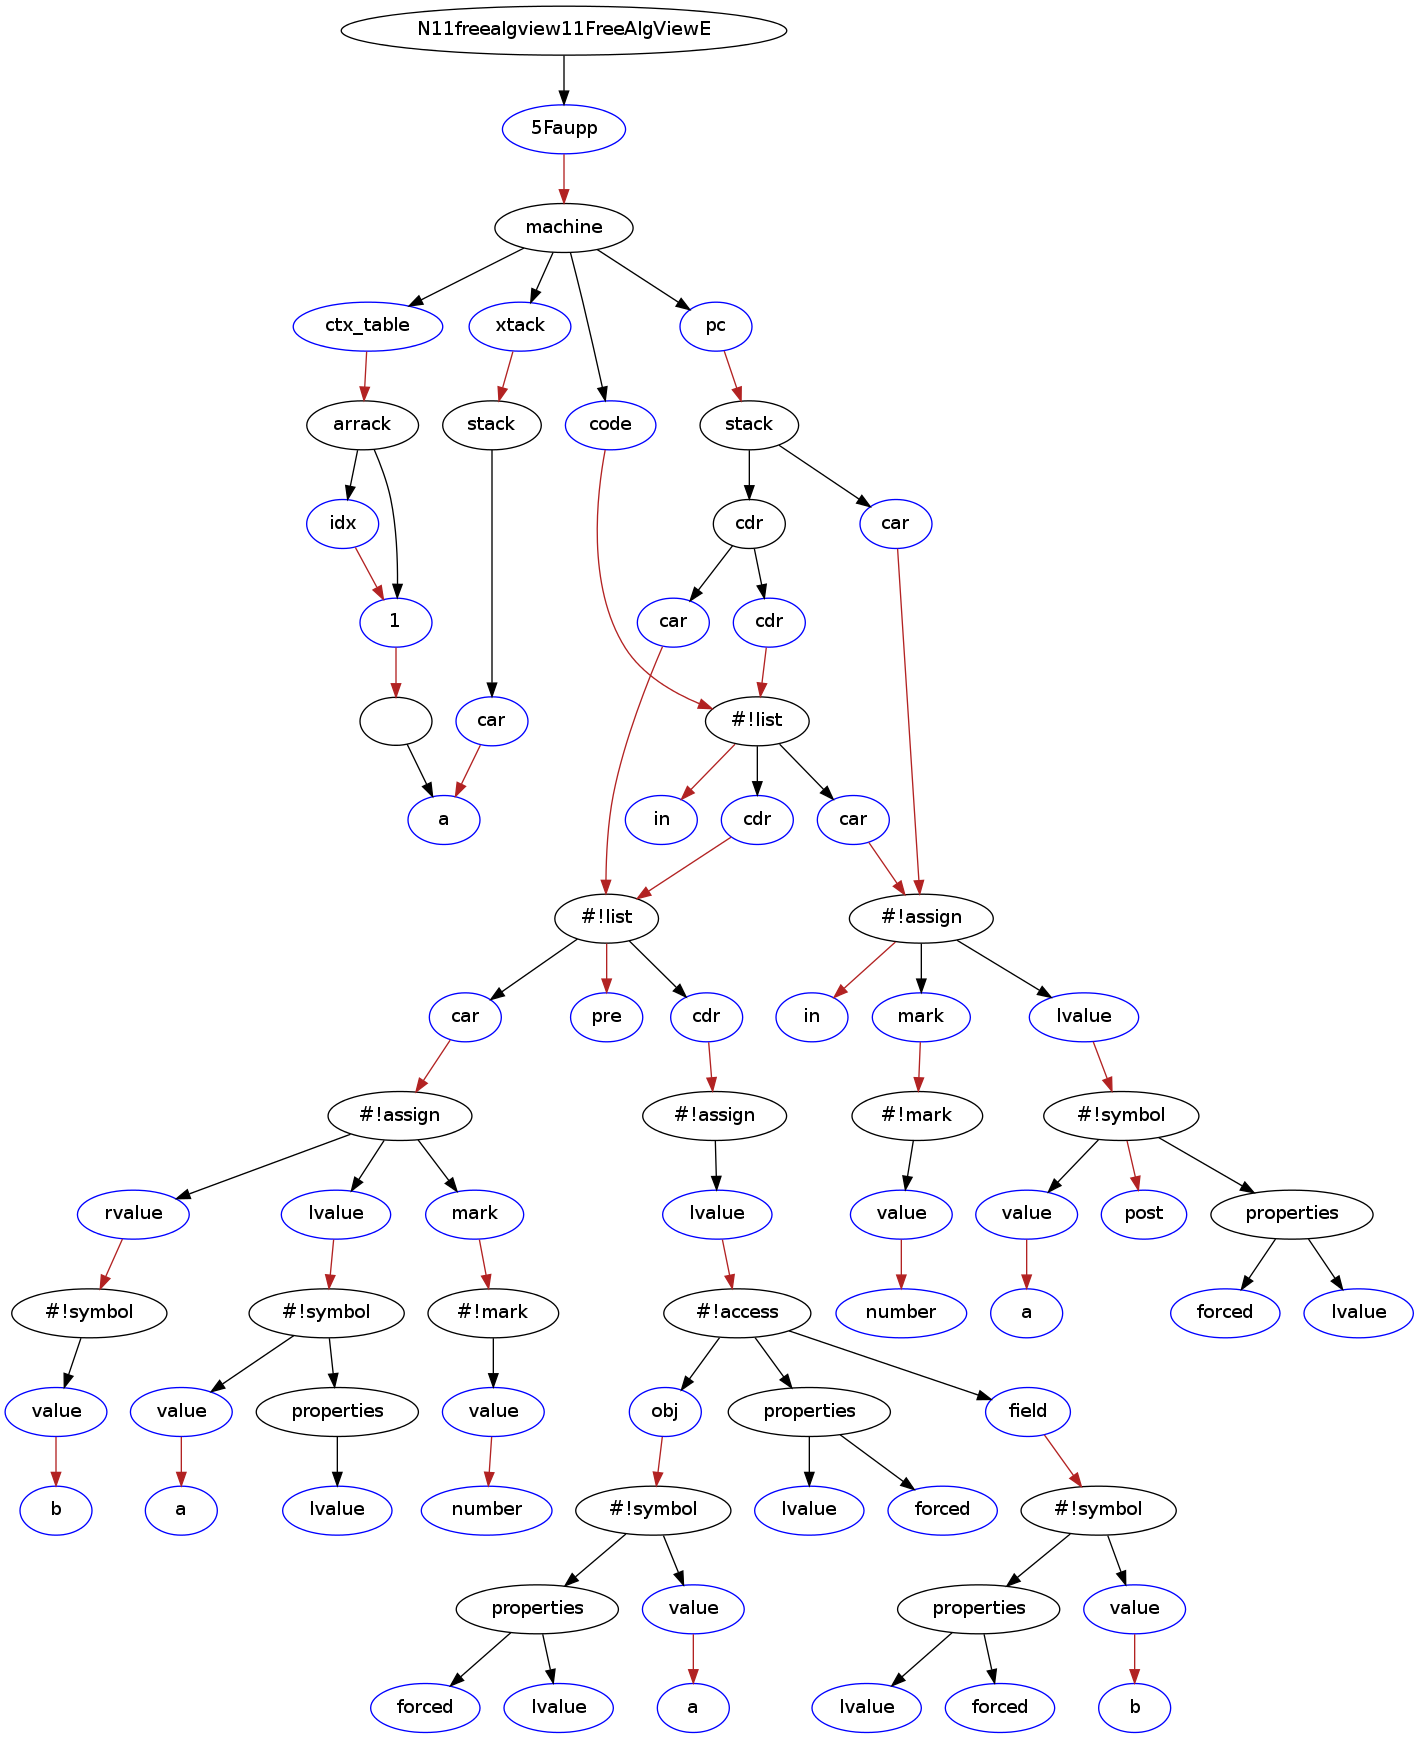
\includegraphics[scale=0.25]{Debugger-out-6.png}
  \caption{Sample output of \texttt{Debugger}}
  \label{fig:deb}
\end{figure}

\begin{figure}[h!]
  \centering
  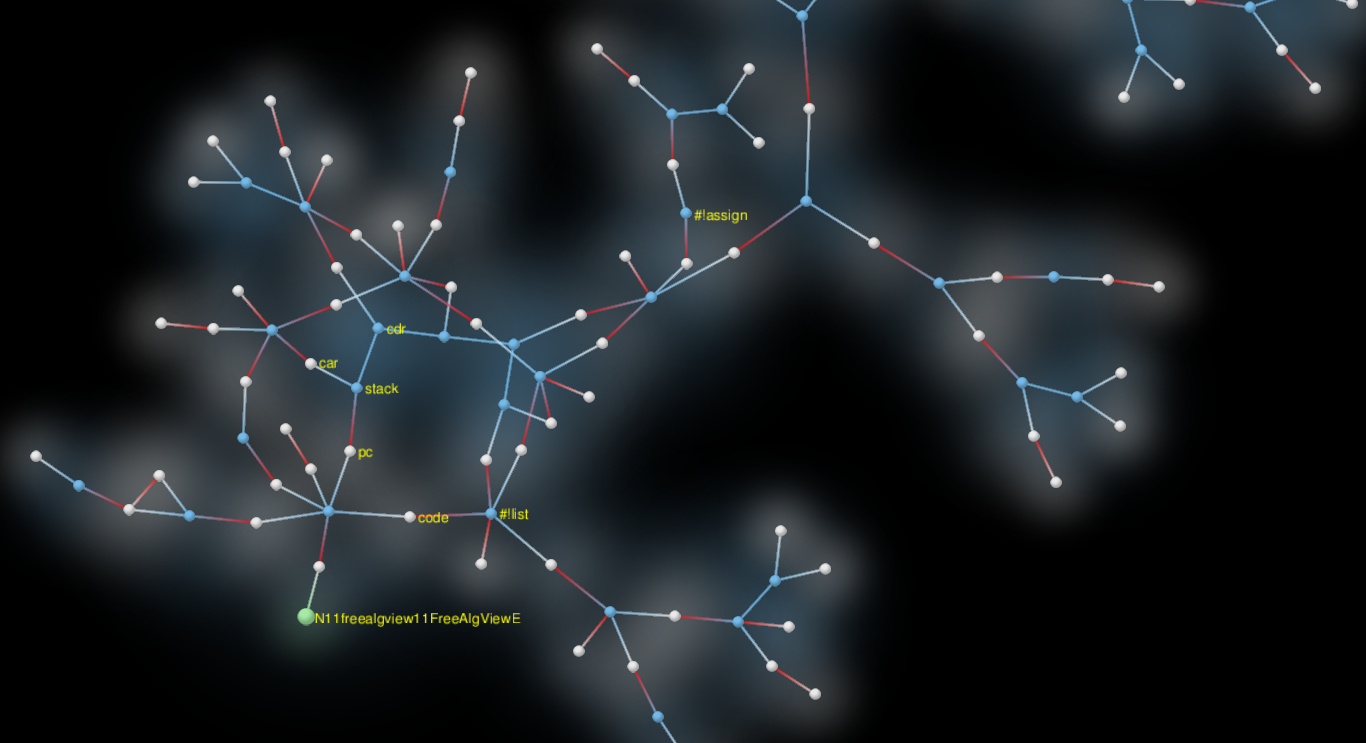
\includegraphics[scale=0.3]{capture.png}
  \caption{Sample output of \texttt{GraphicalDebugger}}
  \label{fig:graphdeb}
\end{figure}

\section{\faupp implementation}
\label{sec:fauppimpl}
In this section, some remarks about the implementation of the interpreter will
be given. Since the implementation of the machine is currently in a very initial
phase of development, this section will be not very long.

Fundamentally, there is five principal nodes (they can be seen in the previous
picture):

\begin{description}
  \item[\texttt{machine}] The root node.
  \item[\texttt{ctx\_table}] The context stack.
  \item[\texttt{code}] The syntax tree.
  \item[\texttt{pc}] The \textit{program counter}. Another stack marking the last
    node being executed and all the unfinished ones.
  \item[\texttt{xtack}] It means eXpressions stack. It is the stack of
    ``anonymous objects''.
\end{description}

In this graphic, red arrows represent references; black arrows, childs; blue
nodes, leafs; and all nodes with names prefixed by \texttt{\#!} are syntax nodes.

The elements above the root represents the application itself (the real root),
and the next one, the interpreter. Their strange names are not due to an error,
they are the mangled names returned by \texttt{typeid(T).name()} for the types
\texttt{FreeAlgView} and \texttt{Faupp}.

Stacks are implemented by means of two children, the first one \texttt{car},
containing the top of the stack, and the second one \texttt{cdr}, with the rest
of the list. The node \texttt{ctx\_table} is an \textit{arrack}, a contraction of
array and stack, since its behaviour is like an stack (FIFO), but its contents
are indexed by number. The top element is maintained by \texttt{idx}. Each
element represent a context of an object, the last one being the most recent. In
this picture there is only one element, with \texttt{idx} pointing to it.

Each \faupp object is a node, with an identifier representing its binding (if
any), a reference to its context (which name represents its mark, if any), and a
number of children to manage the information about overloads (see next section). All
symbols are children of contexts. For example, if the first element of the
context table is looked, it can be seen it contains a reference (read arrow) to
an anonymous node (context without mark), with only a child, \texttt{a}: an
empty object (no context, no mark, no subsymbols; so, no children, no
references).

The uploading of the machine is managed by different function objects being
called in different situations, and modifying the machine accordingly, by means
of \texttt{fnode} operators.

\subsection{Execution process}
\label{ssec:exec}
The general execution process is as following:

\begin{enumerate}
\item \texttt{pc} begins with only one element pointing to the root of the
  syntax tree.
\item The main loop is:

  \begin{enumerate}
  \item Read the top.
  \item Change its state (\texttt{pre} to \texttt{in} and \texttt{in} to
    \texttt{post}).
  \item Go to 1.
  \end{enumerate}

\item The process ends when \texttt{pc} is empty.

\end{enumerate}

The most important thing is the state of each node. \texttt{pre} means previous
step, \texttt{in} inside and \texttt{post}, posterior. Each type of syntax node,
\texttt{\#!list}, \texttt{\#!assign}, \texttt{\#!access}, etc, has different
implementation for each possible state. The fact to have three different states
is for allowing a more granulated evolution of the machine: animations could
want to present an animation of a specific portion of code (a concrete
assignment, a concrete expression, a concrete function call) with a previous
animation before executing it (\texttt{pre}), while executing (\texttt{in}) and
after its executing before popping it from \texttt{pc} (\texttt{post}).

If you see again the machine, the first element of \texttt{pc} is currently an
assignment in ``\texttt{in}'' state. Concretly, it represents \texttt{=> number
  a}. When it was in \texttt{pre} state, its child \texttt{\#!symbol} was pushed
in \texttt{pc} (it was the previous \texttt{pc} top). The execution of this
symbol, throughout all of its states (\texttt{pre}, \texttt{in}, \texttt{post})
was to push its value, \texttt{a}, in \texttt{xtack}, and also in the last
context, since it was forced to do it (the force operator ``\texttt{=>}'' is
represented inside the child \texttt{properties}). You can see the symbol is now
in state \texttt{post} and the assignment being the new top and now ready to be
executed in its \texttt{in} state. Its execution will be: to see there is no
child called rvalue and to pop the \texttt{xtack}, and after its execution the
machine will change its state to \texttt{post}, to pop \texttt{pc}, and to
repeat the complete process for the next element, the second list, which
contains two additional assignments (``\texttt{number a <- b}'' and ``\texttt{=>
  a.b}''). When \texttt{pc} is empty, the program finishes.

\subsection{Symbol management}
When a symbol is executed (with its arguments) the first thing to be done is
search where is the name, and after, to search the correct overload. Lets
me return back to the previous picture. The symbol \texttt{a} is an empty
object. But imagine first its has a context (red arrow to an empty and anonymous
object). If this object would have a base class, this context would have a child
identified by its mark. For $n$ base classes, $n$ children.

When a symbol should be searched, in search from the top of \texttt{ctx\_table}
to bottom, in the same order: base objects, in alphabetical order, own objects,
and if not, repeating the operation in the previous context.

Once the symbol is founded, an overload of it should be selected. Although this
is not yet implemented, the searching algorithm is already designed. Lets me
suppose the following object with the following overloads and the next call:

\begin{faupp2}
  a <- :(@) { /* */ }
       :(double) { /* */ }
       :(int, float) { /* */ }
       :(double, double) { /* */ } (*\label{dd}*)
       :(double, int) { /* */ }
       ;

  => float f;
  => double d;

  a(f, d);
\end{faupp2}

The only compatible overload for this call is the one of line \ref{dd}. How
\faupp find it? In the following picture, a schematic version of the context of
\texttt{a} is depicted:

\begin{figure*}[h!]
\begin{center}
  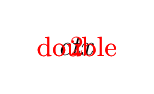
\begin{tikzpicture}[%
      sibling distance=.5cm,
      label/.style={font=\footnotesize\color{red!70!black}}]
    \Tree
        [ .\node{\textit{ctx}}; 0
            [ .1 @ double ]
            \edge[color=red]; [ .\node[color=red]{2}; [ .int float ]
            \edge[color=red];
              [ .\node[color=red]{double}; \edge[color=red];
                                          \node[color=red]{double}; @ ] ] ]
  \end{tikzpicture}
\end{center}
\end{figure*}

Each branch of this tree represents each overload, and each number, the number
of parameters. So, for each number, there is as much branches as overloads with
this number of parameters. In red, is marked the selected overload. Each leaf of
this tree would contain a reference to the code implementing it, but this is
omitted for clarity.

Since we are searching for the overload \texttt{a(float, double)}, we search
first the subtree leaded by \texttt{2}. The next symbol to be searched
correspond to the first parameter, in this case, float. For the next step, we
compare the available types to search the best match. Our inheritance tree is
the following one (list in this case), and \texttt{float} our target (\texttt{@}
represents any object):
\[ \mbox{\texttt{int}} \quad \Rightarrow \quad
   \mbox{\texttt{\textcolor{red}{float}}} \quad \Rightarrow \quad
   \mbox{\texttt{double}} \quad \Rightarrow \quad
   \mbox{\texttt{@}} \]
the best match is then, \texttt{double} (the nearest available ancestor). This
branch has two childs to be compared with \texttt{double}, and the first option
is selected, following the same reasoning, and the correct overload is found and
thereafter executed.

\section{Pending work and new directions}
The projected pending work for the future can be detached in five categories:

\begin{description}
  \item[Short term goals] Finishing the language implementation, reviewing of
    code, basic graphical features and trivial optimizations.
  \item[Medium term goals] Performance with big programs and complex algorithms,
    more graphic features and event treatment, facilities to add textual
    explanations, custom key bindings for users and more control for windows
    layouting.
  \item[Long term goals] Serious benchmarks with huge programs and huge
    animations, automatic searching and loading of suitable animations and
    special facilities for pupils.
  \item[Long long term goals] Integrated text editor, to create algorithms and
    animations inside \fav, Internet access within the application to access to
    third-party algorithms and animations, creation of a web data base,
    exploring algorithms by category, internal wiki to read and edit
    collaboratively complete textual explanations of algorithms (ideal for
    homework) and other Internet-based and social-based features.
  \item[Unsigned long long term goals] Syntax extensibility for domain-specific
    contexts, 3D-features, visualization of mathematical demostrations and a
    integrated graphic editor to facilitate the creation of animations to
    non-programmer users.
\end{description}

\section{Conclusions}
The most important conclusions I have come is about time estimations and
planifications in advance. At the very beginning of my development in October
2012, I spent a lot of time designing my future work, my timeline and my own
directions, in a very formal way, trying to formalize this by project charters
and projects plans. I have spent nearly two months with this work. But at the
very beginning of a project, specially with an invented one, without clear
requirements and without knowing the real nature of my project, and without
clients or a company behind saying you exactly which are the concrete
requirements, is is impossible to know in advance what do you need to do, with
how much time, and most of all, it is impossible to be right.

This could be even counterproductive, because you could want to fit your
schedule all the time with your original plannification, even when, once inside
of your development and fighting against the real nature of your project, you
advice the original plannification wasn't at all suitable. For example, in my
original plannification, my project had two main phases:

\begin{itemize}
\item A first phase where a custom animation should be provided for each algorithm.
\item A second phase where the graphic language should be designed to create
  custom algorithms.
\end{itemize}

Of course, this first phase was for nothing, because custom animations have not
useful value as discussed in the first chapters, and because the work made to
create these ``custom animations'' has been completely deleted, since the
complete structure of \fav has completely change with the introduction of shared
objects, the henfo concept and the new discoveries about the required feature
for \faupp. So, if I join the time consumed in the ``planification phase'' plus
the time consumed making custom animations for nothing, I have spent 5 lovely
and wonderful months: from October to more or less February. The design and
implementation of the basic features of the core module, plus the fnode and
henfo classes lasted about two months: we are now at the end of April. In April
I began to design the language syntax, and this was the most difficult part,
because designing a language requires a completely different mental effort and
way of thinking than designing a database or a software architecture. A new
language, specific for a new situation, needs to solve lots of details, doubts
and ideas that don't go well together, and it is very difficult to be
concentrated and focused with such a chaos. Moreover, to adapt these ideas for
being implemented with a parse generated like \textit{bison} (which does only
implement LL(1) parser, which has some important limitations) forces you to
rethink a lot of things about the language.

The language was finally designed about end of July, but in April I have
though that in about three weeks it will be ready to begin the implementation
(when I say, ``it was designed'', I mean, it was 80\% designed, enough to begin
a serious implementation, because there is yet more think to be defined more
concretely). To this three months (from May to July) I have to erase nearly one
month due to other mandatory activities.

So, my piece of advice is: if you are making a new project without guidance,
don't make your own one, and face soon with the biggest and most difficult
problem of your project, usually the one with the most uncertainty.

\addcontentsline{toc}{section}{References}
\begin{thebibliography}{99}
\bibitem{balsa} Brown, M.H., Sedgewick R. ``A System for Algorithm Animation''.
  \textit{Computer Graphics}. July 1984, pp.177-186.
\bibitem{tango} Stasko, J.T. ``Tango: A Framework and System for Algorithm
  Animation''. \textit{IEEE Computer}. 23, September 1990. pp.27-39.
\bibitem{uuhistle} Juha Sorva, Teemu Sirkiä. \textit{UUhistle. A Program
  Visualization Tool for Introductory Programming Education}. Aalto University
  School of Science and Technology. \url{http://www.uuhistle.org/index.php}.
\bibitem{inaction} Linda Stern, Lee Naish, Harald
  Sondergaard. \textit{Algorithms In Action}. University of Melbourne.
  \url{http://ww2.cs.mu.oz.au/aia/}.
\bibitem{galles} David Galles. \textit{Data Structure Visualization}. University
  of San Francisco. \url{http://www.cs.usfca.edu/~galles/visualization/}.
\bibitem{algoviz} AlgoViz.org. \textit{The Algorithm Visualization Portal}.
  \url{http://algoviz.org/}.
\bibitem{hist} Mei Kei Amy YUNG. ``History of Algorithm
  Animation''. \textit{On-line Animation for a Programming Language
    Course}. 2000.
    \url{http://www.csse.monash.edu.au/hons/projects/2000/Amy.Yung/history.html}.
\end{thebibliography}

\licensesection{Aarón Bueno Villares}{2013}

\end{document}
